%!TEX root =../quadrotorbook.tex
\chapter{Trajectory Generation and Local Planning}
\label{chap:trajectory_planning}

The objective of this chapter is to plan trajectories through a map that represents a cluttered world environment.  The high-level architecture for this chapter is shown in Figure~\ref{fig:planning_architecture}.
\begin{marginfigure}[3in]
  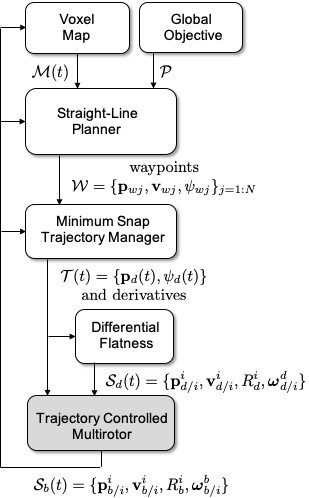
\includegraphics[width=\linewidth]{chap5_trajectory_planning/figures/planning_architecture}
  \caption{The path planning architecture outlined in this chapter.}
  \label{fig:planning_architecture}  
\end{marginfigure}
At the highest level is a voxel representation of the world, local the the multirotor.  The voxel grid will evolve dynamically so that the multirotor always remains in voxel at the center of the map.  A straight-line path planner is then used to plan paths through the voxel map that minimize the distance to the goal location as well as minimize the associated risk.  The output of the straight-line planner is a set of waypoints $\mathcal{W}$ specified as a sequence of desired positions, desired velocities, and desired heading directions.  The waypoints are processed by the {\em minimum-snap trajectory} block to produce a time trajectory of position and heading where the fourth derivative (snap) of the position trajectory is minimized.  The trajectory can be fed directly into the trajectory following framework discussed in Chapter~\ref{chap:trajectory_following}.  However, the framework in Chapter~\ref{chap:trajectory_following} also requires velocity, and angular velocity of the desired multirotor frame.  Those elements are naturally produced by the {\em differential flatness} block shown in Figure~\ref{fig:planning_architecture}.


%----------------------------------
\section{Differential Flatness}
\label{sec:differential_flatness}

Consider the nonlinear system
\begin{equation}\label{eq:flat-system}
\dot{x} = f(x,u),
\end{equation}
where $x$ is the state and $u\in\mathbb{R}^m$ is the control input, and the output mapping
\begin{equation}\label{eq:flat-output}
z = h(x),
\end{equation}
where $z\in\re^p$.  We say that the system~\eqref{eq:flat-system} is differentially flat with flat output $z$ if the following conditions hold~\cite{CowlingYakimenkoWhidborne07}:
\begin{enumerate}
\item The components of $z$ are not differentially related over time.
\item The states $x$ can be written as a function of the flat output and its derivatives, i.e., there exists a function $g_1$, and a finite scalar $m_1$ such that
    \begin{equation}\label{eq:flat-g1}
    x(t) = g_1\left(z(t),\frac{d}{dt}z(t),\cdots,\frac{d^{m_1}}{dt^{m_1}}z(t)\right).
    \end{equation}
\item The control inputs $u$ can be written as a function of the flat output and its derivatives, i.e., there exists a function $g_2$ and a finite scalar $m_2$ such that
    \begin{equation}\label{eq:flat-g2}
    u(t) = g_2\left(z(t),\frac{d}{dt}z(t),\cdots,\frac{d^{m_2}}{dt^{m_2}}z(t)\right).
    \end{equation}
\end{enumerate}

We now show that the multi-rotor system is differentially flat.

\begin{theorem}[Multirotor is Differentially Flat]

Suppose that the multirotor system is given by
\begin{align}
\dot{\pbf}_{d/i}^i &= \vbf_{d/i}^i \label{eq:flat-multirotor-1} \\
\dot{\vbf}_{d/i}^i &= g \ebf_3 + T_d R_d^i \ebf_3 \label{eq:flat-multirotor-2} \\
\dot{R}_d^i &= R_d^i \ss{\omegabf_{d/i}^d}, \label{eq:flat-multirotor-3}
\end{align}
and let $\psi$ be the heading angle, i.e., the body $x$-axis projected onto the inertial $x-y$ plane is 
$\sbf_\psi\doteq (\cos\psi, \sin\psi, 0)^\top$.  

Then the multirotor system is differentially flat with flat outputs $\{\pbf_d(t), \psi_d(t)\} \in\mathbb{R}^3 \times \mathbb{R}$.
\end{theorem}
\begin{proof}
To show that the system is differentially flat, the state variables $\pbf_{d/i}^i$, $\vbf_{d/i}^i$, $R_d^i$ and the input variables $T_d$ and $\omegabf_{d/i}^d$ must all be expressed in terms of the flat outputs $\{\pbf_d(t), \psi_d(t)\}$ and their derivatives.

The position states are directly expressed in the flat outputs as $\pbf_{d/i}^i = \pbf_d(t)$.  The velocity states are directly expressed in the derivative of the flat outputs as $\vbf_{d/i}^i = \dot{\pbf}_d(t)$.

Let the rotation matrix be expressed as 
\[
R_d^i = \begin{pmatrix} \rbf_{1d} & \rbf_{2d} & \rbf_{3d} \end{pmatrix},
\]
where $r_{jd}$ is the $j^{th}$ desired body axis of the multirotor expressed in the inertial frame. Therefore Equation~\eqref{eq:flat-multirotor-2} becomes
\[
T_d r_{3d} = \dot{\vbf}_{d/i}^i - g \ebf_3,
\]
which implies that 
\begin{align*}
T_d &= \norm{\dot{\vbf}_{d/i}^i - g \ebf_3^i} \\
\rbf_{3d} &= \frac{\dot{\vbf}_{d/i}^i - g \ebf_3}{\norm{\dot{\vbf}_{d/i}^i - g \ebf_3}}.
\end{align*}
Therefore the input $T_d$ and the third row of the rotation matrix can be expressed in terms of the flat output as
\begin{align*}
T_d &= \norm{\ddot{\pbf}_d - g \ebf_3} \\
\rbf_{3d} &= \frac{\ddot{\pbf}_d - g \ebf_3}{\norm{\ddot{\pbf}_d- g \ebf_3}}.
\end{align*}
The cross product between the body frame $z$-axis $\rbf_{3d}$ and the heading vector $\sbf_{\psi_d}$ will be in the direction of the body frame $y$-axis and should always be in the inertial $x-y$ plane.  Therefore, $\rbf_{2d}$ is expressed in terms of the flat outputs as
\[
\rbf_{2d} = \frac{\rbf_{3d} \times \sbf_{\psi_d}}{\norm{\rbf_{3d} \times \sbf_{\psi_d}}}.
\]
Since the body frame is a right-handed coordinate system, the body $x$-axis is given by
\[
\rbf_{1d} = \rbf_{2d} \times \rbf_{3d}.
\]
We have shown that $R_d^i$ can be expressed in terms of $\dot{\pbf}_d$ and $\psi_d$.  By differentiating $R_d^i$ it is clear that $\dot{R}_d^i$ can be expressed in terms of $\dot{\pbf}_d$, $\ddot{\pbf}_d$, $\psi_d$ and $\dot{\psi}_d$.  

From Equation~\eqref{eq:flat-multirotor-3}, the angular velocity vector is given by
\[
\omegabf_{d/i}^d = \left(R_d^{i\top} \dot{R}_d^i\right)^\vee. 
\]

Summarizing, the states and outputs are expressed in the flat outputs and their derivatives as
\begin{align*}
\pbf_{d/i}^i(\pbf_d) &= \pbf_d(t) \\
\vbf_{d/i}^i(\dot{\pbf}_d) &= \dot{\pbf}_d(t) \\
\rbf_{3d}(\ddot{\pbf}_d) &= \frac{\ddot{\pbf}_d - g \ebf_3}{\norm{\ddot{\pbf}_d - g \ebf_3}} \\
\rbf_{2d}(\ddot{\pbf}_d, \psi_d) &= \frac{\rbf_{3d} \times \sbf_{\psi_d}}{\norm{\rbf_{3d} \times \sbf_{\psi_d}}} \\
\rbf_{1d}(\ddot{\pbf}_d, \psi_d) &= \rbf_{2d} \times \rbf_{3d} \\
R_d^i(\ddot{\pbf}_d, \psi_d) &= \begin{pmatrix} \rbf_{1d} & \rbf_{2d} & \rbf_{3d} \end{pmatrix} \\
T_d(\ddot{\pbf}_d) &= \norm{\ddot{\pbf}_d - g \ebf_3} \\	
\omegabf_{d/i}^d(\ddot{\pbf}_d, \dddot{\pbf}_d, \psi_d, \dot{\psi}_d) &= (R_d^{i\top}\dot{R}_d^i)^\vee.
\end{align*}

Since all states and inputs can be expressed in terms of the flat outputs and their derivatives, the system is differentially flat.
\end{proof}

The inclusion of the induced drag term in the dynamics does not change the differential flatness property, although it does change equations expressions for the states and input variables.  The complete derivation is given in~\cite{FaesslerFranchiScaramuzza18.pdf}.


%\subsection{Differential Flatness of Quadrotor Dynamics Subject to Rotor Drag, RAL, 2018}
%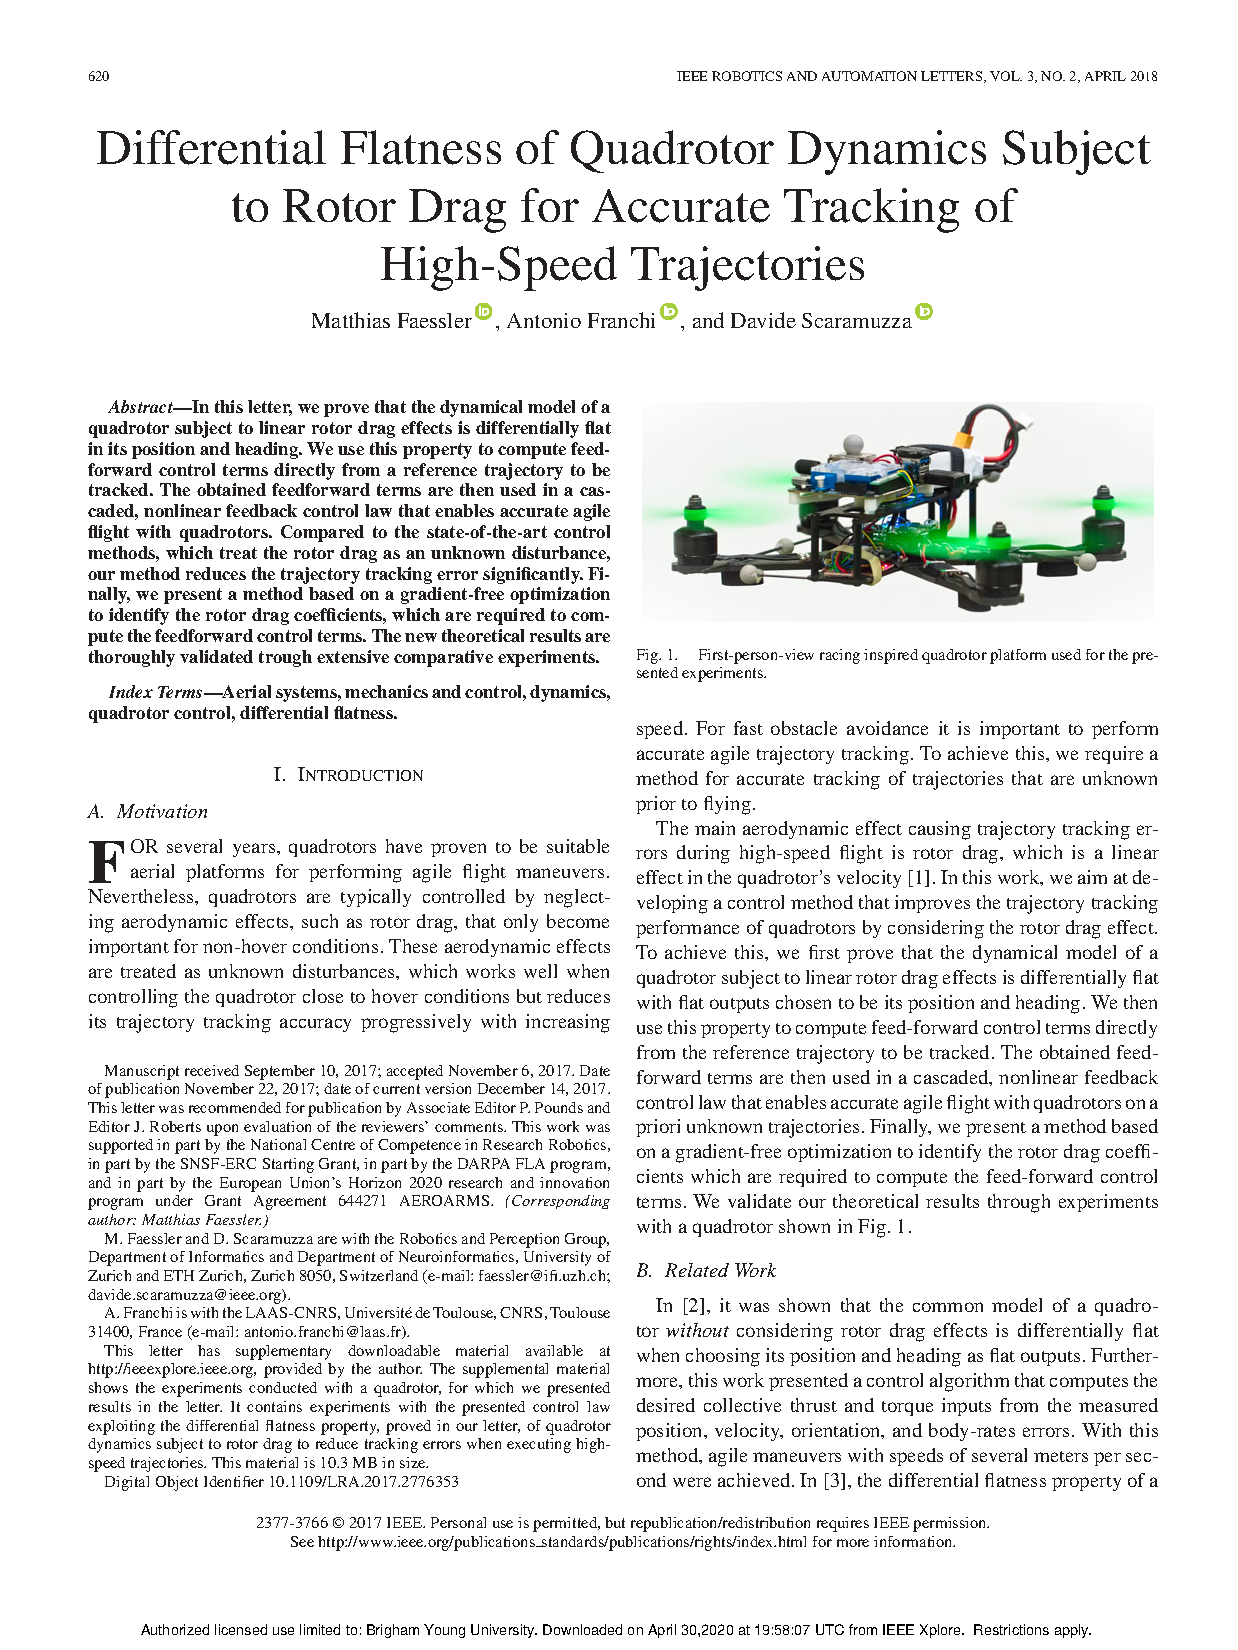
\includepdf[pages=-,scale=.8,pagecommand={}]{chap5_trajectory_planning/papers/FaesslerFranchiScaramuzza18.pdf}




%++++++++++++++++++++++++++++++++++++++++++++++++++++++++++++++
\subsection{Analytic calculation of desired angular velocity}
Author: Jacob Willis

%
%\usepackage[utf8]{inputenc}
%\usepackage{amsmath}
%\usepackage{amssymb}
%\usepackage{graphicx}
%\graphicspath{ {./figs/} }
%
%% \usepackage{theorem}
%\usepackage{amsthm}
%\newtheorem{theorem}{Theorem}
%\newtheorem{property}{Property}
%\def\proof{\hspace{1em}{\it Proof: }}
%\def\endproof{\hspace*{\fill}~$\blacksquare$\par\endtrivlist\unskip}
%
%\newtheorem*{remark}{Remark}
%
%\usepackage[hidelinks]{hyperref}
%\usepackage{color}
%\newcommand{\rwbcomment}[1]{{\color{red} RWB: #1}}
%\newcommand{\jbwcomment}[1]{{\color{blue} JBW: #1}}
%%\usepackage{cite}
%\usepackage{multirow}
%\usepackage[margin=1in]{geometry}
%
%\usepackage{biblatex}
%\addbibresource{bib_willis/references.bib}
%
%%\DeclareMathOperator{\mod}{mod}
%\DeclareMathOperator{\floor}{floor}
%\DeclareMathOperator{\rank}{rank}
%\DeclareMathOperator{\vspan}{span}
%\DeclareMathOperator*{\argmin}{arg min}
%
%\title{\LARGE Analytic Derivative of the Desired Rotation Matrix for Control}
%\author{Jacob Willis}
%
%\begin{document}
%\maketitle

Rather than numerically differentiating $R_d^i$ as described in Section~\ref{sec:numerical_differentiation_of_R}, this section shows how to find the time derivative of $R_d^i$ analytically.
First, recall that
\begin{equation}
	R_d^i = \begin{pmatrix} \mathbf{r}_{1d} & \mathbf{r}_{2d}&  \mathbf{r}_{3d} \end{pmatrix}
\end{equation}
and therefore that
\begin{equation}
	\dot{R}_d^i = \begin{pmatrix} \dot{\mathbf{r}}_{1d} & \dot{\mathbf{r}}_{2d} & \dot{\mathbf{r}}_{3d} \end{pmatrix}.
\end{equation}

To proceed, we need the following two properties.
\begin{property}
	The time derivative of the cross product of two time-dependent vectors $\mathbf{x}$ and $\mathbf{y}$ is
	\begin{equation}
		\label{eq:cross_derivative}
		\frac{d}{dt} (\mathbf{x} \times \mathbf{y}) = \dot{\mathbf{x}} \times \mathbf{y} + \mathbf{x} \times \dot{\mathbf{y}}
	\end{equation}
\end{property}
\proof
This is easiest to see by recalling that $\mathbf{x} \times \mathbf{y} = \mathbf{x}^\wedge \mathbf{y}$ where the result follows from the product rule.
\endproof

\begin{property} \label{prop:derivative_of_normal_vector}
	The time derivative of a normalized vector $\frac{\mathbf{x}}{\|\mathbf{x}\|}$ is
	\begin{equation}
		\label{eq:norm_derivative}
		\frac{d}{dt} \left(\frac{\xbf}{\norm{\xbf}}\right) = \Pi_{\frac{\xbf}{\norm{\xbf}}} \frac{\dot{\xbf}}{\norm{\xbf}},
	\end{equation}
	where $\Pi_{\nbf} \doteq I-\nbf\nbf^\top$ is the projection operator on to the plane orthogonal to the unit vector $\nbf$.
\end{property}
\proof
	By the quotient rule, we have
	\begin{equation}
		\frac{d}{dt} \frac{\mathbf{x}}{\|\mathbf{x}\|} = \frac{\dot{\mathbf{x}} \|\mathbf{x}\| - \mathbf{x} \frac{d}{dt}(\|\mathbf{x}\|)}{\|\mathbf{x}\|^2}.
	\end{equation}
	Now,
	\begin{align}
		\frac{d}{dt} \|\mathbf{x}\| 
		= \frac{d}{dt} \sqrt{\mathbf{x}^\top \mathbf{x}} 
		= \frac{1}{2 \sqrt{\mathbf{x}^\top \mathbf{x}}} (\dot{\mathbf{x}}^\top \mathbf{x} + \mathbf{x}^\top \dot{\mathbf{x}})
		= \frac{\dot{\mathbf{x}}^\top \mathbf{x}}{\|\mathbf{x}\|}
	\end{align}
	Plugging in, we get
	\begin{equation}
		\frac{d}{dt} \frac{\mathbf{x}}{\|\mathbf{x}\|} = \frac{\dot{\mathbf{x}}}{\|\mathbf{x}\|} - \mathbf{x} \frac{\dot{\mathbf{x}}^\top \mathbf{x}}{\|\mathbf{x}\|^3}.
	\end{equation}
	Rearranging gives
	\[
	\frac{d}{dt} \frac{\mathbf{x}}{\|\mathbf{x}\|} =  \left(I-\frac{\xbf}{\norm{\xbf}}\frac{\xbf^\top}{\norm{\xbf}}\right)\frac{\dot{\xbf}}{\norm{\xbf}}.
	\]

\endproof

The third column of the rotation matrix is given by
\begin{equation}
	\mathbf{r}_{3d} = - \frac{\ddot{\mathbf{p}}_d - g \mathbf{e}_3 - K_p \tilde{\mathbf{p}} - K_d \dot{\tilde{\mathbf{p}}}} {\norm{\ddot{\pbf}_d - g \ebf_3 - K_p \tilde{\pbf} - K_d \dot{\tilde{\pbf}}}}.
\end{equation}
Therefore, using the properties above we get that
\[
\dot{\rbf}_{3d} = \Pi_{\rbf_{3d}} \left(\frac{-\dddot{\pbf}_d + K_p \dot{\tilde{\pbf}} + K_d \ddot{\tilde{\pbf}}}{\norm{\ddot{\pbf}_d - g \ebf_3 - K_p \tilde{\pbf} - K_d \dot{\tilde{\pbf}}}}\right).
\]
The second column of the rotation matrix is given by
\[
\rbf_{2d} = \frac{\rbf_{3d}\times\sbf_{\psi_d}}{\norm{\rbf_{3d}\times\sbf_{\psi_d}}},
\]
which implies that
\[
\dot{\rbf}_{2d} = \Pi_{\rbf_{2d}}\left(\frac{\dot{\rbf}_{3d}\times\sbf_{\psi_d}+\dot{\psi}_d\rbf_{3d}\times (-\sin\psi_d,  \cos\psi_d, 0)^\top }{\norm{\rbf_{3d}\times\sbf_{\psi_d}}}\right).
\]
The first column of the rotation matrix is given by
\[
\rbf_{1d} = \rbf_{2d}\times\rbf_{3d},
\]
which implies that
\[
\dot{\rbf}_{1d} = \dot{\rbf}_{2d}\times\rbf_{3d} + \rbf_{2d}\times \dot{\rbf}_{3d}.
\]
The angular velocity can now be calculated as
\[
\omegabf_{d/i}^d(\pbf_d, \dot{\pbf}_d, \ddot{\pbf}_d, \dddot{\pbf}_d, \psi_d, \dot{\psi}_d) = \left[\begin{pmatrix}\rbf_{1d} & \rbf_{2d} & \rbf_{3d}\end{pmatrix}^\top \begin{pmatrix} \dot{\rbf}_{1d} & \dot{\rbf}_{2d} & \dot{\rbf}_{3d} \end{pmatrix}\right]^\vee.
\]





%----------------------------------
\section{An Introduction to b-Spline}


The objective of these notes is to explore spline methods for robotic applications. In general, the position of a robot in Euclidian space can be described by a time parametrized trajectory $\mathbf{p}(t)\in\mathbb{R}^3$, $t\in[a,b]$.  The time parametrized trajectory can be parameterized using a weighted sum of basis function as
\[
\mathbf{p}(t) = \sum_{m=0}^{N} \cbf_m \phi_m(t),
\]
where $\cbf_m\in\mathbb{R}^n$, and $\phi_m(t)$ are a set of basis functions.  For example, the basis functions could be the set of polynomial power function $\phi_m(t) = t^m/m!$, or the set of sinusoidal function $\phi_m(t) = \sin(\frac{2\pi m}{N}t)$.  The disadvantage of both the polynomial power functions and sinusoidal functions is that the basis functions are defined for all $t\in[a,b]$ and so each control points $\mathbf{c}_m$ influences the entire trajectory.  Another disadvantage is that a large number of basis functions may be required to represent complicated trajectories.  

In these notes, we will use B-spline basis functions which have a number of very nice properties that we will explore.  In particular, a {\em B-spline} trajectory has the following form
\[
\mathbf{p}(t) = \sum_{m=0}^{N} \cbf_m b_m^k(t;\mathbf{t}),
\]
where $\cbf_m\in\mathbb{R}^n$ are the control points,  $\mathbf{t}=(\tau_0, \tau_1, \tau_2, \dots, \tau_T)$ are called the knot points where $i<j \implies \tau_i\leq \tau_j$, and $b_m^k(t;\mathbf{t})$ are the B-spline basis functions of order $k$. The spline trajectories will be defined for $t$ in the span of the knot points, i.e., $t\in[\tau_0, \tau_T]$.  

Section~\ref{sec:b-spline-basis-functions} defines the B-spline basis function $b_m^k(t; \mathbf{t})$ and describes some of their properties that will be useful for path planning and for estimation.
Section~...
% overview of other sections

%---------------------------------------------------------------
\subsection{B-Spline Basis Functions}
\label{sec:b-spline-basis-functions}

The B-spline basis function are defined by the recursive formula:
\begin{align}
b_m^1(t; \mathbf{t}) &= \begin{cases} 1 & \text{~if~} \tau_m \leq t \leq \tau_{m+1} \\ 
 									 0 & \text{~otherwise} 
 					   \end{cases} 
	\label{eq:spline_basis_definition_0}\\	
b_m^k(t; \mathbf{t}) &= w_m^k(t; \mathbf{t}) b_m^{k-1}(t; \mathbf{t}) + \left[1-w_{m+1}^k(t; \mathbf{t})\right] b_{m+1}^{k-1}(t; \mathbf{t}),
	\label{eq:spline_basis_definition_k} \\
w_m^k(t; \mathbf{t}) &= \begin{cases}
                      		\frac{t-\tau_m}{\tau_{m+k}-\tau_m}, & \tau_{m+k}\neq \tau_m \\
                      		0, & \text{~otherwise} 
                        \end{cases}.
\end{align}

%+++++++++++++++++++++++++++++++
\par\noindent{\bf First order basis}

For example, if the knot vector is given by
\[
\mathbf{t} = [\tau_0, \tau_1, \tau_2] \defeq [0, 1, 2],
\]
then there are two basis function of order $k=1$ given by
\begin{align*}
b_0^1(t; \mathbf{t}) &= \begin{cases} 1 & \text{~if~} \tau_0 \leq t \leq \tau_1 \\ 
 									 0 & \text{~otherwise} 
 			\end{cases}
\\ 
b_1^1(t; \mathbf{t}) &= \begin{cases} 1 & \text{~if~} \tau_1 \leq t \leq \tau_2 \\ 
 									 0 & \text{~otherwise}
 			\end{cases}
\end{align*}
where $b_0^1(t)$ and $b_1^0=1(t)$ are shown in Figure~\ref{fig:spline_basis_0}.
\begin{figure}[hbt]
  \centering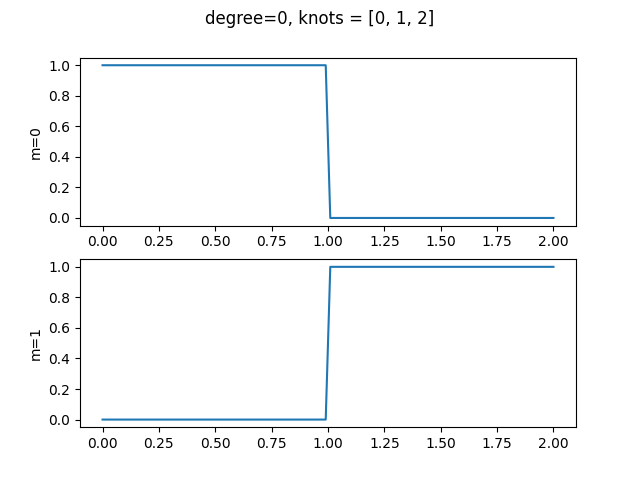
\includegraphics[width=0.5\textwidth]{./chap5_trajectory_planning/figures/spline_basis_0}
  \caption{First order spline basis}
  \label{fig:spline_basis_0}  
\end{figure}
Note that $b_1^1(t; \mathbf{t}) = b_0^1(t-1; \mathbf{t})$, or in other words, all first order basis functions are shifted versions of the central first order basis function $b_0^1(t; \mathbf{t})$.  Additional first order basis function can be defined by expanding the knot vector to $\mathbf{t}=[0, \dots, M]$, where $b_m^1(t; \mathbf{t})= b_0^1(t-m; \mathbf{t})$ for $m\leq M$.

\clearpage


%+++++++++++++++++++++++++++++++
\par\noindent{\bf Second order basis}

If the knot vector is given by
\[
\mathbf{t} = [\tau_0, \tau_1, \tau_2, \tau_3, \tau_4] \defeq [0, 0, 1, 2, 2],
\]
then there are $2k-1=3$ unique basis function of order $k=2$ given by
\begin{align*}
b_0^2(t; \mathbf{t}) &= \frac{t-\tau_0}{\tau_1-\tau_0} b_0^1(t;\mathbf{t}) + \frac{\tau_2-t}{\tau_2-\tau_1}b_1^1(t; \mathbf{t}) 
	= \begin{cases} 0   & \text{~if~} t_0=0 \leq t \leq t_1=0 \\
				    1-t & \text{~if~} t_1=0 \leq t \leq t_2=1 \\ 
 	  \end{cases}
\\ 
b_1^2(t; \mathbf{t}) &= \frac{t-\tau_1}{\tau_2-\tau_1} b_1^1(t;\mathbf{t}) + \frac{\tau_3-t}{\tau_3-\tau_2}b_2^1(t; \mathbf{t})
	= \begin{cases} t & \text{~if~} t_1=0 \leq t \leq t_2=1 \\ 
 									2-t & t_2=1 \leq t \leq t_3=2 \\
 									0 & \text{~otherwise}
 					    \end{cases}
\\ 
b_2^2(t; \mathbf{t}) &= \frac{t-\tau_2}{\tau_3-\tau_2} b_2^1(t;\mathbf{t}) + \frac{\tau_4-t}{\tau_4-\tau_3}b_3^1(t; \mathbf{t})
	= \begin{cases} t-1 & \text{~if~} t_2=1 \leq t \leq t_3=2 \\ 
 					0 & \text{~if~} t_3=2 \leq t \leq t_4=2 \\
 	  \end{cases}
\end{align*}
where $b_0^2(t; \mathbf{t})$, $b_1^2(t; \mathbf{t})$, and $b_2^2(t; \mathbf{t})$ are shown on the left in Figure~\ref{fig:spline_basis_1}.
\begin{figure}[hbt]
  \centering
  	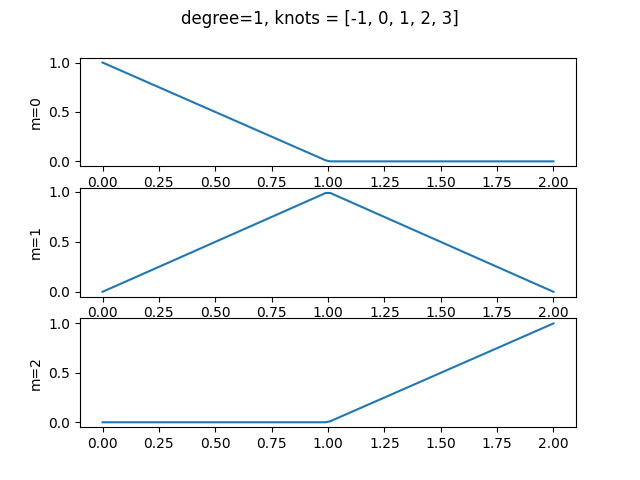
\includegraphics[width=0.45\textwidth]{./chap5_trajectory_planning/figures/spline_basis_1}
  	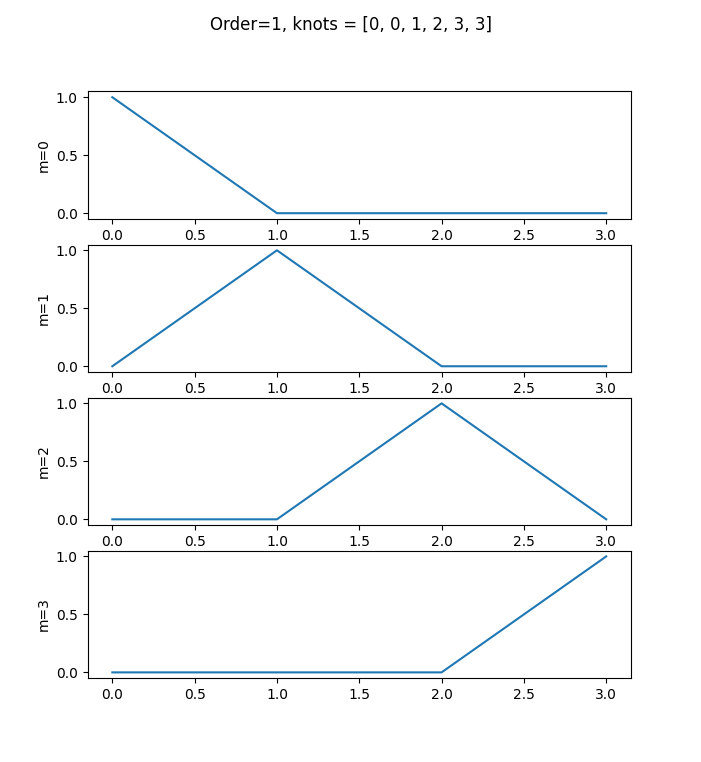
\includegraphics[width=0.45\textwidth]{./chap5_trajectory_planning/figures/spline_basis_1_extra_knot}
  \caption{Second order spline basis}
  \label{fig:spline_basis_1}  
\end{figure}
If the knot vector is expanded by one time unit to
\[
\mathbf{t}' = [\tau_0, \tau_1, \tau_2, \tau_3, \tau_4, \tau_5] \defeq [0, 0, 1, 2, 3, 3],
\]
then there are still only three unique basis vectors, but 
$b_2^2(t; \mathbf{t}')$ is a shifted version $b_1^2(t; \mathbf{t})$ and $b_3^2(t; \mathbf{t}')$ is a shifted version $b_2^2(t; \mathbf{t})$, as shown on the right in Figure~\ref{fig:spline_basis_1}.

\clearpage


%+++++++++++++++++++++++++++++++
\par\noindent{\bf Third order basis}

If the knot vector is given by
\[
\mathbf{t} = [\tau_0, \tau_1, \tau_2, \tau_3, \tau_4, \tau_5, \tau_6, \tau_7, \tau_8] \defeq [0, 0, 0, 1, 2, 3, 3, 3],
\]
then there are $2k-1=5$ unique basis function of order $k=3$ given by
\begin{align*}
b_0^3(t; \mathbf{t}) &= \frac{t-\tau_0}{\tau_2-\tau_0} b_0^2(t;\mathbf{t}) + \frac{\tau_3-t}{\tau_3-\tau_1}b_1^2(t; \mathbf{t}) 
	= \begin{cases} (1-t)^2   & \text{~if~} 0 \leq t \leq 1 \\
				    0 & \text{~otherwise~}  \\ 
 	  \end{cases}
\\ 
b_1^3(t; \mathbf{t}) &= \frac{t-\tau_1}{\tau_3-\tau_1} b_1^2(t;\mathbf{t}) + \frac{\tau_4-t}{\tau_4-\tau_2}b_2^2(t; \mathbf{t})
	= \begin{cases} t(2-\frac{3}{2}t) & \text{~if~} 0 \leq t \leq 1 \\ 
 									\frac{(2-t)^2}{2} & 1 \leq t \leq 2 \\
 									0 & \text{~otherwise}
 					    \end{cases}
\\ 
b_2^3(t; \mathbf{t}) &= \frac{t-\tau_2}{\tau_4-\tau_2} b_2^2(t;\mathbf{t}) + \frac{\tau_5-t}{\tau_5-\tau_3}b_3^2(t; \mathbf{t})
	= \begin{cases} \frac{t^2}{2} & \text{~if~} 0 \leq t \leq 1 \\ 
 					-\frac{3}{2}t^2 + \frac{7}{2}t - \frac{3}{2} & \text{~if~} 1 \leq t \leq 2 \\
 					\frac{(3-t)^2}{2} & \text{~if~} 2 \leq t \leq 3 \\
 					0 & \text{~otherwise}
 	  \end{cases}
\\ 
b_3^3(t; \mathbf{t}) &= \frac{t-\tau_2}{\tau_4-\tau_2} b_2^2(t;\mathbf{t}) + \frac{\tau_5-t}{\tau_5-\tau_3}b_3^2(t; \mathbf{t})
	= \begin{cases} \frac{(t-1)^2}{2} & \text{~if~} 1 \leq t \leq 2 \\ 
 					-\frac{3}{2}t^2 + \frac{15}{2}t-\frac{15}{2} & \text{~if~} 2 \leq t \leq 3 \\
 					0 & \text{~otherwise}
 	  \end{cases}
\\ 
b_4^3(t; \mathbf{t}) &= \frac{t-\tau_2}{\tau_4-\tau_2} b_2^2(t;\mathbf{t}) + \frac{\tau_5-t}{\tau_5-\tau_3}b_3^2(t; \mathbf{t})
	= \begin{cases} (t-2)^2 & \text{~if~} 2 \leq t \leq 3 \\ 
 					0 & \text{~otherwise}
 	  \end{cases}.	   	  
\end{align*}
The the unique third order basis function are shown on the left in Figure~\ref{fig:spline_basis_2}.
\begin{figure}[hbt]
  \centering
  	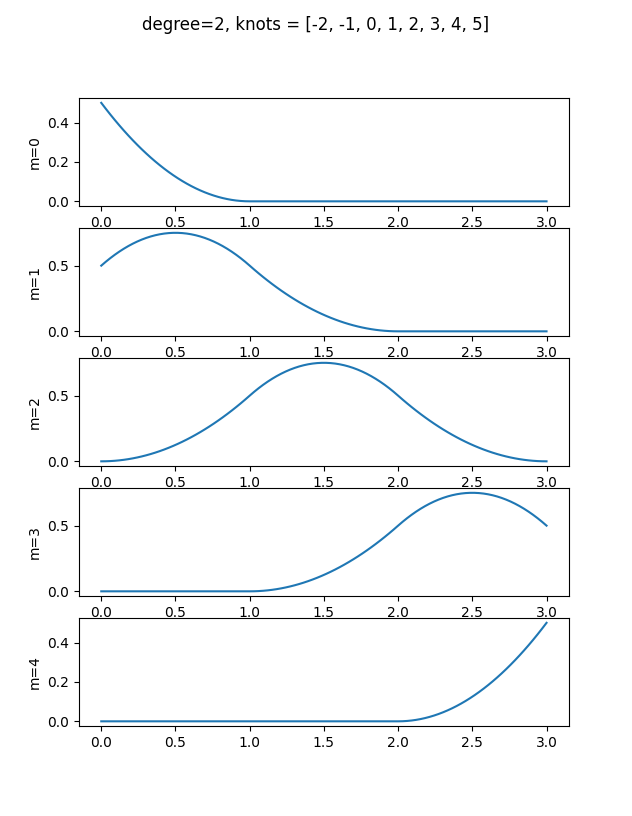
\includegraphics[width=0.45\textwidth]{./chap5_trajectory_planning/figures/spline_basis_2}
  	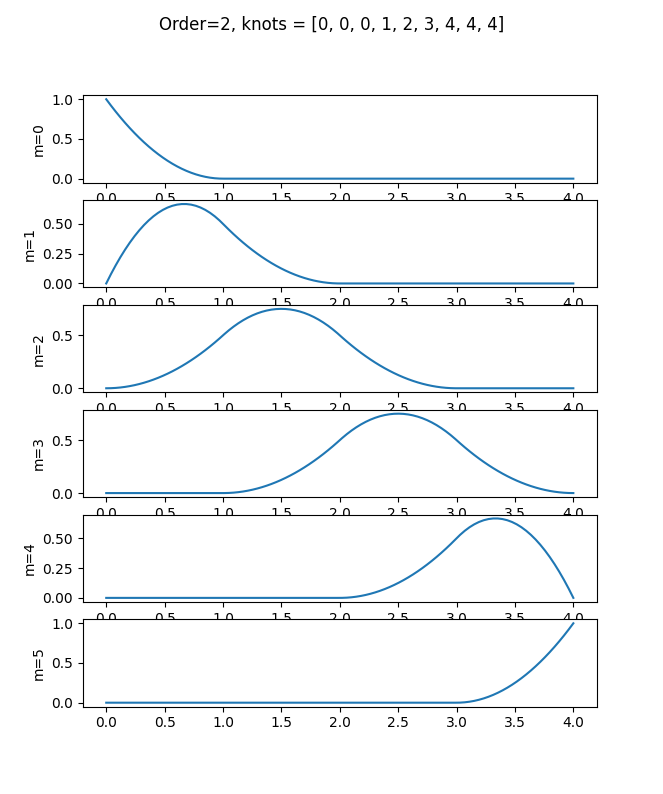
\includegraphics[width=0.45\textwidth]{./chap5_trajectory_planning/figures/spline_basis_2_extra_knot}
  \caption{Third order spline basis}
  \label{fig:spline_basis_2}  
\end{figure}
Expanding the knot vector by one time unit to 
\[
\mathbf{t}' = [\tau_0, \tau_1, \tau_2, \tau_3, \tau_4, \tau_5] \defeq [0, 0, 0, 1, 2, 3, 4, 4, 4],
\]
still results in $2k-1$ unique basis vectors, but $b_3^3(t; \mathbf{t}')$ is a right-shifted version of $b_2^3(t; \mathbf{t})$, and $b_4^3(t; \mathbf{t}')$ and $b_5^3(t; \mathbf{t})$ are a right-shifted versions of $b_3^3(t; \mathbf{t}')$ and $b_4^3(t; \mathbf{t})$, as shown on the right in Figure~\ref{fig:spline_basis_2}.

Similarly, the unique fourth order and ninth order basis functions are shown in Figures~\ref{fig:spline_basis_3} and~\ref{fig:spline_basis_8} respectively.

\begin{figure}[hbt]
  \centering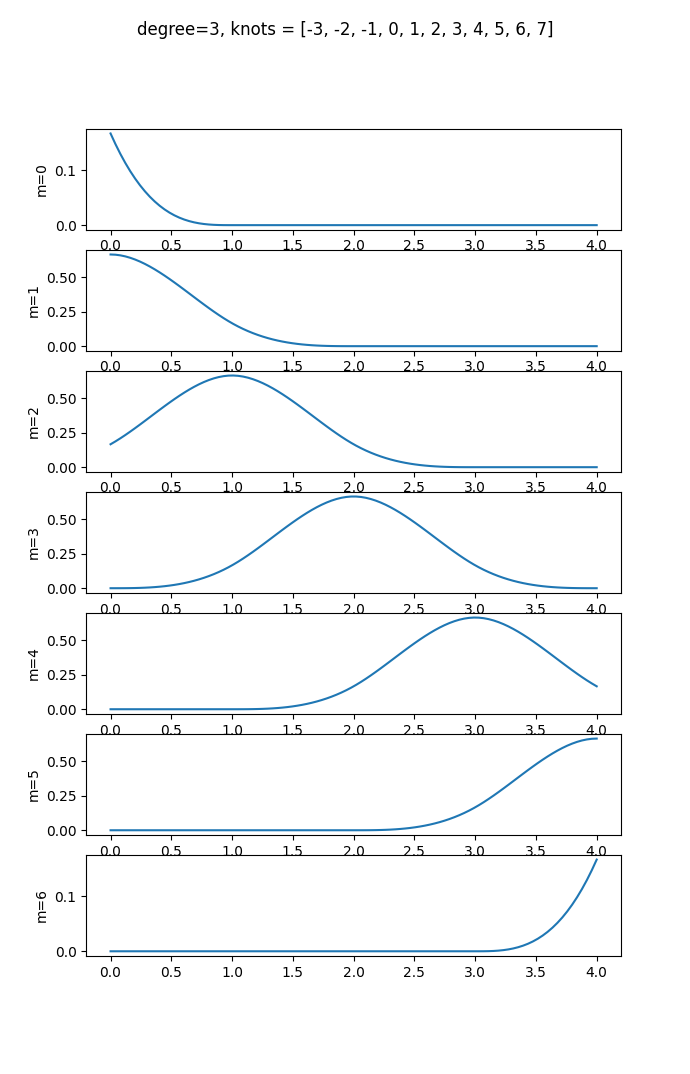
\includegraphics[width=0.99\textwidth]{./chap5_trajectory_planning/figures/spline_basis_3}
  \caption{Fourth order spline basis}
  \label{fig:spline_basis_3}  
\end{figure}

\begin{figure}[hbt]
  \centering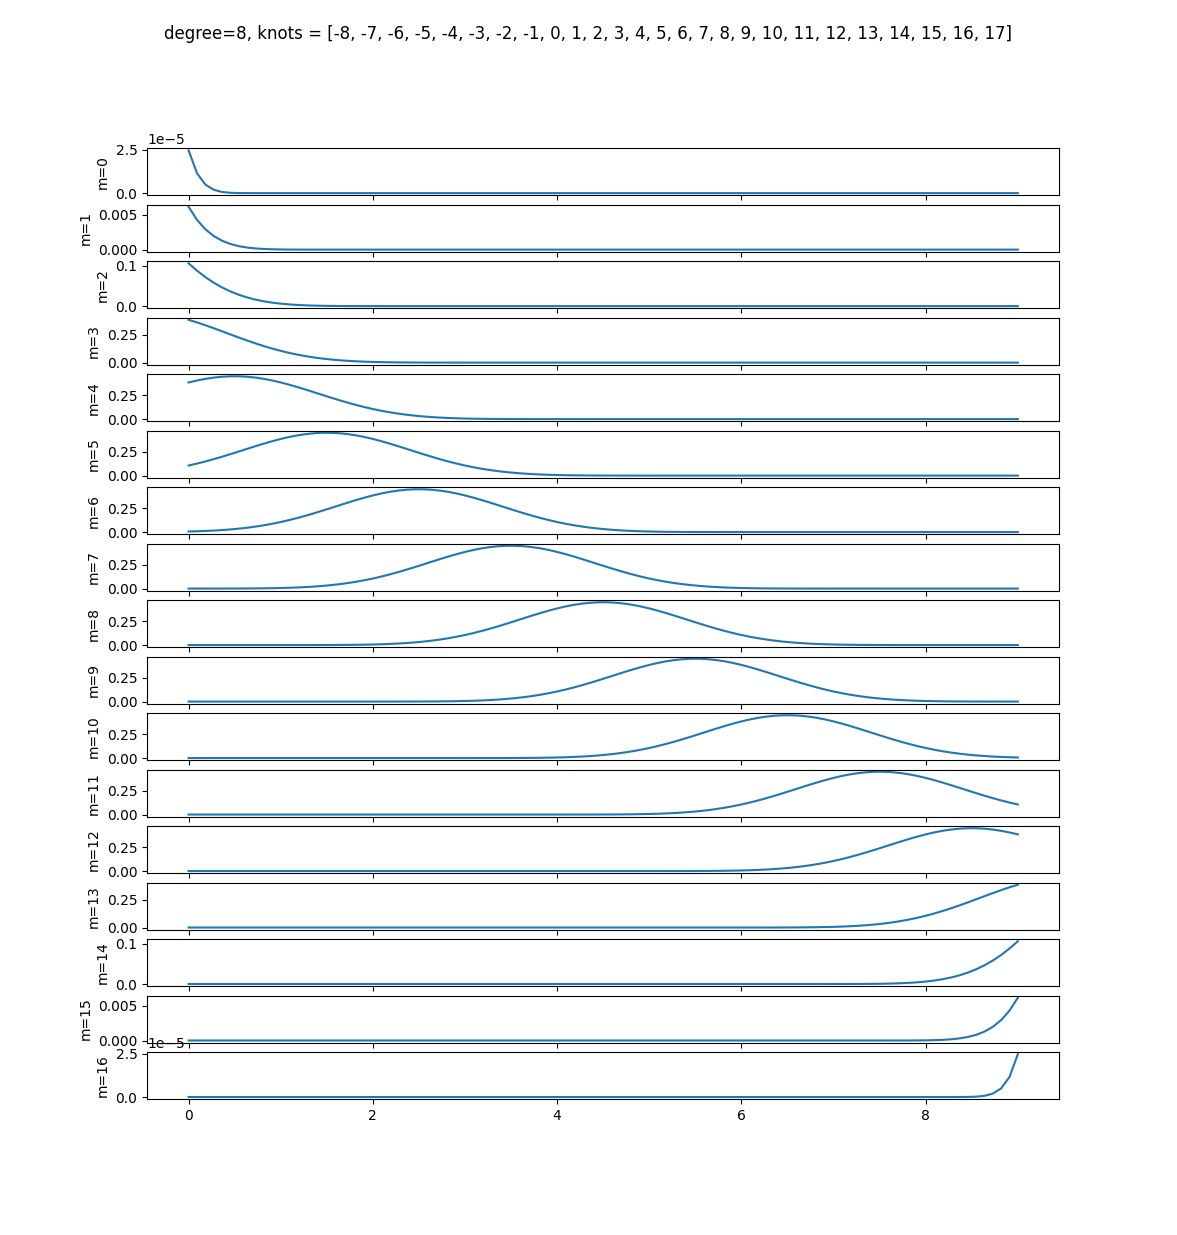
\includegraphics[width=0.99\textwidth]{./chap5_trajectory_planning/figures/spline_basis_8}
  \caption{Ninth order spline basis}
  \label{fig:spline_basis_8}  
\end{figure}

\clearpage

%---------------------------------------------------------------
\par\noindent{\bf Shift and Scale Invariance of the Knot Sequence}

\begin{lemma} \label{lem:basis_are_shift_invariant}
Given an arbitrary knot sequence
\[
\mathbf{t} = [\tau_0, \tau_1, \dots \tau_T],
\]
an arbitrary time shift $\Delta$, and the one-sequenc $\mathbf{1}\defeq[1, 1, \dots, 1]$, the B-spline basis functions are shift invariant in the sense that
if 
\[
\mathbf{t} + \Delta\mathbf{1} = [\tau_0+\Delta, \tau_1+\Delta, \dots \tau_T+\Delta]
\]
then
\[
b_j^k(t; \mathbf{t}+\Delta\mathbf{1}) = b_j^k(t-\Delta; \mathbf{t}),
\]
i.e., shifting the knot sequence forward in time is identical to shifting the original B-spline forward in time.
\end{lemma}
\begin{proof}
When the order is $k=1$, then equation~\eqref{eq:spline_basis_definition_0} gives
\begin{align*}
	b_j^1(t; \mathbf{t}+\Delta\mathbf{1}) &= \begin{cases} 1 & \text{~if~} \tau_j+\Delta \leq t \leq \tau_{j+1}+\Delta \\ 
 									 				   0 & \text{~otherwise} 
 					   					 \end{cases} \\
 					   				   &= \begin{cases} 1 & \text{~if~} \tau_j \leq t-\Delta \leq \tau_{j+1} \\ 
 									 				   0 & \text{~otherwise} 
 					   					 \end{cases} \\ 	
 					   				   &= b_j^1(t-\Delta; \mathbf{t}).
\end{align*}
Assuming that the statement holds when the order is $k-1\geq 0$, we get from 
Equation~\eqref{eq:spline_basis_definition_k} that
\begin{align*}
b_j^k(t; \mathbf{t}+\Delta\mathbf{1}) &= \frac{t-\tau_j-\Delta}{\tau_{j+k}+\Delta-
\tau_j-\Delta} b_j^{k-1}(t; \mathbf{t}+\Delta\mathbf{1}) + \frac{\tau_{j+k+1}+\Delta-t}{\tau_{j+k+1}+\Delta-\tau_{j+1}-\Delta} b_{j+1}^{k-1}(t; \mathbf{t}+\Delta\mathbf{1}) \\
&= \frac{(t-\Delta)-\tau_j}{\tau_{j+k}-
\tau_j} b_j^{k-1}(t-\Delta; \mathbf{t}) + \frac{\tau_{j+k+1}-(t-\Delta)}{\tau_{j+k+1}-\tau_{j+1}} b_{j+1}^{k-1}(t-\Delta; \mathbf{t}) \\
&= b_j^k(t-\Delta; \mathbf{t}).
\end{align*}
The proof therefore follows by induction.
\end{proof}


\begin{lemma}\label{lem:bases_are_scale_invariant}
Given an arbitrary knot sequence
\[
\mathbf{t} = [\tau_0, \tau_1, \dots \tau_T]
\]
and an arbitrary scaling constant $\alpha\in\mathbb{R}$, the B-spline basis functions are scale invariant in the sense that
if 
\[
\alpha\mathbf{t} = [\alpha\tau_0, \alpha\tau_1, \dots \alpha\tau_T]
\]
then
\[
b_j^k(t; \alpha\mathbf{t}) = b_j^k(t/\alpha; \mathbf{t}),
\]
i.e., scaling the knot sequence by $\alpha$ is identical to time scaling the original B-spline by $\frac{1}{\alpha}$.
\end{lemma}
\begin{proof}
When the order is $k=1$, then equation~\eqref{eq:spline_basis_definition_0} gives
\begin{align*}
	b_j^1(t; \alpha\mathbf{t}) &= \begin{cases} 1 & \text{~if~} \alpha\tau_j \leq t \leq \alpha\tau_{j+1} \\ 
 									 				   0 & \text{~otherwise} 
 					   					 \end{cases} \\
 					   				   &= \begin{cases} 1 & \text{~if~} \tau_j \leq \frac{t}{\alpha} \leq \tau_{j+1} \\ 
 									 				   0 & \text{~otherwise} 
 					   					 \end{cases} \\ 	
 					   				   &= b_j^1(t/\alpha; \mathbf{t}).
\end{align*}
Assuming that the statement holds when the order is $k-1\geq 0$, we get from 
Equation~\eqref{eq:spline_basis_definition_k} that
\begin{align*}
b_j^k(t; \alpha\mathbf{t}) &= \frac{t-\alpha\tau_j}{\alpha\tau_{j+k}-
\alpha\tau_j} b_j^{k-1}(t; \alpha\mathbf{t}) + \frac{\alpha\tau_{j+k+1}-t}{\alpha\tau_{j+k+1}-\alpha\tau_{j+1}} b_{j+1}^{k-1}(t; \alpha\mathbf{t}) \\
&= \frac{(t/\alpha)-\tau_j}{\tau_{j+k}-
\tau_j} b_j^{k-1}(t/\alpha; \mathbf{t}) + \frac{\tau_{j+k+1}-(t/\alpha)}{\tau_{j+k+1}-\tau_{j+1}} b_{j+1}^{k-1}(t/\alpha; \mathbf{t}) \\
&= b_j^k(t/\alpha; \mathbf{t}).
\end{align*}
The proof therefore follows by induction.
\end{proof}


%---------------------------------------------------------------
\subsection{Uniform B-Splines}

In the previous section we saw that there is a relationship between the knot point vector $\mathbf{t}$ and the basis functions.  We say that the knot vector $\mathbf{t}$ is {\em uniform} if the knot values are equally spaced, i.e., it has form
\begin{multline*}
\mathbf{t} = [\underbrace{\tau_0-(k-1)\Delta, \dots, \tau_0-\Delta,}_{(k-1)-terms} \\
			 \underbrace{\tau_0, \tau_0+\Delta, \tau_0+2\Delta, \dots, \tau_0+M\Delta,}_{M+1-terms} \\
			 \underbrace{\tau_0+(M+1)\Delta, \dots, \tau_0+(M+k-1)\Delta}_{(k-1)-terms}],	
\end{multline*}
where $\Delta>0$ and $M\geq k$.  
For example, the following knot vectors are uniform:
\begin{align*}
	(t_0=0, k=3, \Delta=1, M=3):\quad & \mathbf{t} = [-2, -1, \vdots~ 0, 1, 2, 3, \vdots~ 4, 5] \\
	(t_0=-3, k=4, \Delta=1, M=5):\quad & \mathbf{t} = [-6, -5, -4,\vdots~  -3, -2, -1, 0, 1, 2, \vdots~ 3, 4, 5] \\
	(t_0=0, k=4, \Delta=\frac{1}{5}, M=5):\quad & \mathbf{t} = [-\frac{3}{5}, -\frac{2}{5}, -\frac{1}{5}, \vdots~  0, \frac{1}{5}, \frac{2}{5}, \frac{3}{5}, \frac{4}{5}, 1, \vdots~  \frac{6}{5}, \frac{7}{5}, \frac{8}{5}].	
\end{align*}

 We say that the knot vector $\bar{\mathbf{t}}$ is {\em uniform and clamped} (the overbar is used to denote clamped) if the knot values are equally spaced and the first and last $(k-1)$-terms are repeated, i.e., it has form
\begin{multline*}
\bar{\mathbf{t}} = [\underbrace{\tau_0, \tau_0, \dots, \tau_0,}_{(k-1)-terms} \\
			 \underbrace{\tau_0, \tau_0+\Delta, \tau_0+2\Delta, \dots, \tau_0+M\Delta,}_{M+1-terms} \\
			 \underbrace{\tau_0+M\Delta, \dots, \tau_0+M\Delta}_{(k-1)-terms}],	
\end{multline*}
where $\Delta>0$ and $M\geq k$.  

For example, the following knot vectors are clamped and uniform:
\begin{align*}
	(t_0=0, k=3, \Delta=1, M=3):\quad & \bar{\mathbf{t}} = [0, 0, \vdots~ 0, 1, 2, 3, \vdots~ 3, 3] \\
	(t_0=-3, k=4, \Delta=1, M=5):\quad & \bar{\mathbf{t}} = [-3, -3, -3, \vdots~ -3, -2, -1, 0, 1, 2, \vdots~ 2, 2, 2] \\
	(t_0=0, k=4, \Delta=\frac{1}{5}, M=5):\quad & \bar{\mathbf{t}} = [0, 0, 0, \vdots~ 0, \frac{1}{5}, \frac{2}{5}, \frac{3}{5}, \frac{4}{5}, 1, \vdots~ 1, 1, 1].	
\end{align*}
Similarly, the knot vectors shown in Figures~\ref{fig:spline_basis_0}, \ref{fig:spline_basis_1}, \ref{fig:spline_basis_2}, \ref{fig:spline_basis_3}, and~\ref{fig:spline_basis_8} are all clamped and uniform.  

The length of uniform, and uniform and clamped knot vectors is 
\[
\text{length}(\mathbf{t}) = M+1 + 2(k-1) = M+2k-1,
\]
and, in both cases, the time interval of interest is $t\in[t_0, t_0+M\Delta$, where there are $M$ evenly spaced time intervals. 

B-splines associated with uniform knot vectors are called uniform b-splines, and they are only valid on the time interval $t\in[t_0, t_0+M\Delta]$, similarly B-splines associated with uniform and clamped knot vectors are called uniform and clamped b-splines, and they are also only valid on the time interval $t\in[t_0, t_0+M\Delta]$.

In the rest of this tutorial, we will focus on the knot vectors
\begin{align}
	\mathbf{t}^k_M &\defeq [-(k-1), \dots, -1, 0, 1, 2, \dots, M, M+1, \dots, M+k-1],
		\label{eq:knot_vector_t_M} \\ 
	\bar{\mathbf{t}}^k_M &\defeq [\underbrace{0, 0, \dots, 0}_{(k-1)-\text{terms}}, 0, 1, 2, \dots, M, \underbrace{M, \dots, M}_{(k-1)-\text{terms}}], 
	\label{eq:knot_vector_tbar_M}
\end{align}
and use Lemmas~\ref{lem:basis_are_shift_invariant} and~\ref{lem:bases_are_scale_invariant} to adapt the results to any desired time interval by shifting and scaling.

There are several important properties of the B-spline basis functions for uniform and clamped knot vectors, which we will lay out in the next several lemmas.

\begin{lemma} \label{lem:shifted_central_basis}
Let $\mathbf{t}_M^k$ be the uniform knot vector defined in Equation~\eqref{eq:knot_vector_t_M} with $M\geq k$, then the basis function $b_k^{k-1}(t; \mathbf{t}_M^k)$ plays a central role in the sense that
\[
	b_{k-1+m}^{k}(t; \mathbf{t}_M^k) = b_{k-1}^k(t-m; \mathbf{t}_M^k), \qquad m=-k, \dots, M-1.
\]
\end{lemma}
\begin{proof}
From Equation~\eqref{eq:spline_basis_definition_0} we give that
\begin{align*}
	b_m^1(t; \mathbf{t}_M^k) &= \begin{cases} 1 & \text{~if~} m \leq t \leq m+1 \\ 
 									 		  0 & \text{~otherwise} 
 					   			\end{cases} 
 					   		\\
 					   		 &= \begin{cases} 1 & \text{~if~} 0 \leq t-m \leq 1 \\ 
 									 		  0 & \text{~otherwise} 
 					   			\end{cases} 
 					   		\\
 					   		&= b_0^1(t-m; \mathbf{t}_M^k).
\end{align*}
Suppose that $b_{k-2+m}^{k-1}(t; \mathbf{t}_M^k) = b_{k-2}^{k-1}(t-m; \mathbf{t}_M^k)$, then
\begin{align*}
b_{k-1+m}^{k}(t; \mathbf{t}_M^k) 
	&= \frac{t-(k+m)}{m+2k-(m+k)} b_{k-1+m}^{k-1}(t; \mathbf{t}_M^k) + \frac{m+2k+1-t}{m+2k+1-(m+k+1)} b_{k+m}^{k-1}(t; \mathbf{t}_M^k),
	\\	
	&= \frac{(t-m)-k)}{k} b_{k-1}^{k-1}(t-m; \mathbf{t}_M^k) + \frac{2k+1-(t-m)}{k} b_{k1}^{k-1}(t-m; \mathbf{t}_M^k),
	\\
	&= b_{k-1}^k(t-m; \mathbf{t}_M^k).
\end{align*}
Therefore, the lemma holds by induction.
\end{proof}



\begin{lemma} \label{lem:nonzero_basis_vectors}
	Let $\mathbf{t}_M^k$ be a uniform clamped knot vector defined in Equation~\eqref{eq:knot_vector_t_M} with $M\geq k$.
	Then there are exactly $M+k-1$ non-zero basis function of order $k$, namely $b_m^k(t;\mathbf{t}_M^k)$, $m=0, \dots, M+k-1$.
	Furthermore, the basis of support for $b_m^k(t;\mathbf{t}_M^k)$, i.e., the time interval where $b_m^k(t;\mathbf{t}_M^k)$ is non-zero is given by
		\[
				b_m^k(t;\mathbf{t}_M^k) \neq 0 
				\quad \text{~if~} \quad
				\begin{cases}
				t \in [0, m+1] & 0\leq m \leq k-1 \\
				t \in [m-k+1, m+1] & k \leq m \leq M-1 \\
				t \in [m-k+1, M] & M \leq m \leq M+k-2
				\end{cases}.
		\]	
\end{lemma}
\begin{proof}  The proof follows from a careful, but straight-forward accounting using Equations~\eqref{eq:spline_basis_definition_0} and~\eqref{eq:spline_basis_definition_k}.	
\end{proof}

A graphical depiction of the region of support for the set of basis functions $\{b_m^k(t;\mathbf{t}_M^k)\}_{m=0}^{M+k-2}$ is shown in Figure~\ref{fig:region_of_support} for $k=4$ and $M=8$.
\begin{figure}[hbt]
  \centering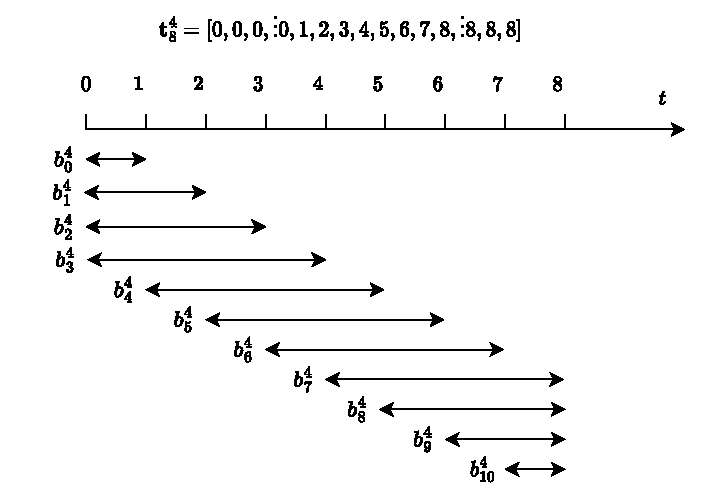
\includegraphics[width=0.99\textwidth]{./chap5_trajectory_planning/figures/region_of_support}
  \caption{Region of support for the B-spline basis functions of order $k=4$ with knot vector $\mathbf{t}_8^4$.}
  \label{fig:region_of_support}  
\end{figure}

\begin{lemma} \label{lem:basis_vectors_sum_to_1}
	Let $\mathbf{t}_M^k$ be a uniform clamped knot vector defined in Equation~\eqref{eq:knot_vector_t_M} with $M\geq k$. For any instant of time $t\in[0,M]$, the basis vectors at that time sum to unity, i.e., for $t\in[0, M]$,
	\[
	\sum_{m=0}^{M+k-2} b_m^k(t; \mathbf{t}_M^k) = 1.
	\]
\end{lemma}
\begin{proof}  The proof again follows from a careful, but straight-forward accounting using Equations~\eqref{eq:spline_basis_definition_0} and~\eqref{eq:spline_basis_definition_k}.	
\end{proof}

\begin{definition}
Let $\{\cbf_0, \cbf_1, \dots, \cbf_{M+k-2}\}$ be a set of control point vectors in $\mathbb{R}^n$, and let $\mathbf{t}_M^k$ be a clamped and uniform knot vector, then the function 
\begin{equation}\label{eq:clamped_uniform_spline}
\mathbf{p}(t) = \sum_{m=0}^{M+k-2} \cbf_m b_m^k(t; \mathbf{t}_M^k), \qquad t\in[0, M]
\end{equation}
is said to be a $k^{th}$ order clamped and uniform B-spline. 
\end{definition}

One of the most important properties of B-splines is the so-called finite-support property, which states that at any instant of time, only a few control points influence the B-spline.  This property is formalized in the following lemma.
\begin{lemma}\label{lem:finite_num_control_points}
	Let $\mathbf{t}_M^k$ be a uniform clamped knot vector defined in Equation~\eqref{eq:knot_vector_t_M} with $M\geq k$. If $0\leq j < M$ is an integer, then for any instant of time $t\in[j, j+1]\subset [0, M]$ we have that
	\[
	\mathbf{p}(t) = \sum_{m=0}^{M+k-2} \cbf_m b_m^k(t; \mathbf{t}_M^k) = \sum_{m=j}^{j+k-1} \cbf_m b_m^k(t; \mathbf{t}_M^k).
	\]
	In other words, over the interval $t\in[j, j+1]$ there are only $k$ control points that influence $\mathbf{p}(t)$, namely
	$\{\cbf_j, \dots, \cbf_{j+k-1}\}$.
\end{lemma}
\begin{proof}
The proof follows directly from Lemma~\ref{lem:nonzero_basis_vectors}.	
\end{proof}



Another important property of B-splines, is that the spline $\mathbf{p}(t)$ is contained in the convex hull of its supporting control points.  
\begin{definition}
We say that the vector $\xbf$ is in the convex hull of the vectors $\{\mathbf{q}_1, \dots, \mathbf{q}_n\}$ if 
\[
\xbf = \sum_{j=1}^n \alpha_j \mathbf{q}_j, \qquad \text{where} \qquad \sum_{j=1}^n \alpha_j = 1.
\]	
\end{definition}

\begin{lemma}\label{lem:spline_in_convex_hull}
	Let $\mathbf{t}_M^k$ be a uniform or uniform clamped knot vector defined in Equation~\eqref{eq:knot_vector_t_M} with $M\geq k$. If $0\leq j < M$ is an integer, then for any instant of time $t\in[j, j+1]\subset [0, M]$ we have that the B-spline
	\[
	\mathbf{p}(t) = \sum_{m=0}^{M+k-2} \cbf_m b_m^k(t; \mathbf{t}_M^k) = \sum_{m=j}^{j+k-1} \cbf_m b_m^k(t; \mathbf{t}_M^k)
	\]
	is in the convex hull of the control points $\{\cbf_j, \dots, \cbf_{j+k-1}\}$.
\end{lemma}
\begin{proof}
	The lemma follows from Lemma~\ref{lem:basis_vectors_sum_to_1} and~\ref{lem:finite_num_control_points}.
\end{proof}
Lemma~\ref{lem:spline_in_convex_hull} is an important result for path planning since we can guarantee collision-free paths by simply checking that the convex hull of control points is collision free.


To simplify notation we will stack the basis function in a vector as
\begin{equation}\label{eq:basis_vector}
\bbf_M^k(t) \defeq \begin{pmatrix} b_0^k(t;\mathbf{t}_M^k) \\ b_1^k(t;\mathbf{t}_M^k) \\ \vdots \\ b_{M+k-2}^k(t;\mathbf{t}_M^k) \end{pmatrix}, 
\end{equation}
and the control points as a matrix 
\[
\Cbf = \begin{pmatrix} \cbf_0 & \cbf_1 & \dots & \cbf_{M+k-2} \end{pmatrix}
\]
allowing Equation~\eqref{eq:clamped_uniform_spline} to be written as
\[
\mathbf{p}(t) = \Cbf \bbf_M^k(t), \qquad t\in[0, M].
\]
Given the shift and scale invariance of the B-spline basis functions, $\mathbf{p}(t)$ can be shifted and scaled to represent functions over arbitrary finite time intervals.

%For parameterized paths $\mathbf{p}(\sigma)$, where the path parameter $\sigma\in[0,1]$ we set the knot vector as $\frac{1}{M}\mathbf{t}_{M}^k$
%and the parameterized B-spline is given by
%\[
%\mathbf{p}(\sigma) = \Cbf \bbf_M^k(\sigma; \frac{1}{M}\mathbf{t}_{M}^k), \qquad \sigma\in[0, 1].
%\]
%Abusing notation, we will use $\bbf_M^k(\sigma)$ to mean $\bbf_M^k(\sigma; \frac{1}{M}\mathbf{t}_{M}^k)$, and parameterized paths with always be defined for $\sigma\in[0,1]$

%---------------------------------------------------------
\par\noindent{\bf SciPy BSpline library}
The SciPy library has a B-spline library.  

The following commands will create a cubic spline.
\begin{lstlisting}
import numpy as np
from scipy.interpolate import BSpline
	
	
def uniform_clamped_knots(k, M, t0=np.inf, tf=np.inf):
    # k is the order, M is the number of time intervals
    knots = [0] * k + list(range(0, M + 1)) + [M] * k
    knots = np.asarray(knots)  # convert knots to an NP array
    if t0 != np.inf:
        if (tf != np.inf) & (tf > t0):
            knots = (tf-t0)/M * knots
        knots = knots + t0
    return knots	

t0 = 1 # initial time
tf = 5 # final time
k = 3  # spline order
M = 3  # number of time intervals
knots = uniform_clamped_knots(k=order, M=M, t0=t0, tf=tf)
# need M+k control points
ctrl_pts = np.array([[0, 0, 0],  
                     [0, 1, 0],
                     [0, 0, 1],
                     [0, 1, 1],
                     [1, 1, 0],
                     [1, 1, 1]])
spl = BSpline(t=knots, c=ctrl_pts, k=order)
plot_spline(spl)
\end{lstlisting}

Where {\tt plot\_spline} is given below.
\begin{lstlisting}
from math import ceil
from scipy.interpolate import BSpline
import matplotlib.pyplot as plt

def plot_spline(spl):
    t0 = spl.t[0]  # first knot is t0
    tf = spl.t[-1]  # last knot is tf
    # number of points in time vector so spacing is 0.01
    N = ceil((tf - t0)/0.01)
    t = np.linspace(t0, tf, N)  # time vector
    position = spl(t)
    # 3D trajectory plot
    fig = plt.figure(1)
    ax = fig.add_subplot(111, projection='3d')
    # plot control points (convert YX(-Z) -> NED)
    ax.plot(spl.c[:, 1], spl.c[:, 0], -spl.c[:, 2],
            '-o', label='control points')
    # plot spline (convert YX(-Z) -> NED)
    ax.plot(position[:, 1], position[:, 0], -position[:, 2],
            'b', label='spline')
    ax.legend()
    ax.set_xlabel('x', fontsize=16, rotation=0)
    ax.set_ylabel('y', fontsize=16, rotation=0)
    ax.set_zlabel('z', fontsize=16, rotation=0)
    #ax.set_xlim3d([-10, 10])
    plt.show()
\end{lstlisting}

The resulting spline is shown in Figure~\ref{fig:example_spline_curve}.
\begin{figure}[hbt]
  \centering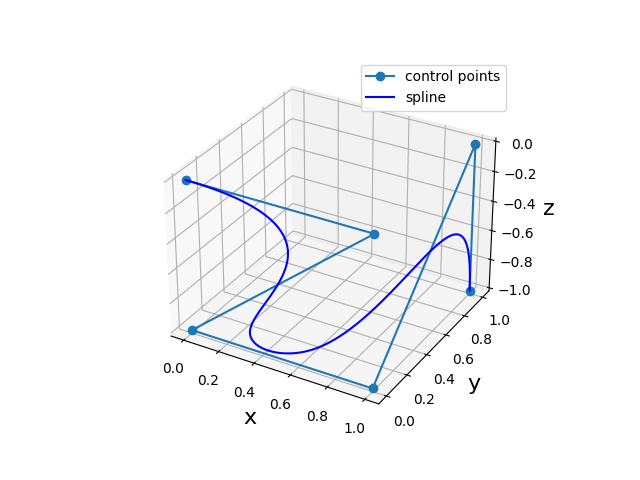
\includegraphics[width=0.5\textwidth]{./chap5_trajectory_planning/figures/example_spline_curve}
  \caption{Example spline curve}
  \label{fig:example_spline_curve}  
\end{figure}

%+++++++++++++++++++++++++++++++
\subsection{Derivatives of B-splines}

We begin this section by noting that the basis functions and the knot vector do not have to be of the same order.  In fact, if the knot vector has higher order than the basis functions, then the first several basis functions will simply be zero.  
For example, let $\mathbf{t}_3^3 = [0, 0\vdots, 0, 1, 2, 3, \vdots 3, 3]$, then from Equation~\eqref{eq:spline_basis_definition_0} $b_0^1(t; \mathbf{t}_3^3)$, $b_1^1(t; \mathbf{t}_3^3)$, $b_5^1(t; \mathbf{t}_3^3)$, $b_1^1(t; \mathbf{t}_3^3)$, and $b_5^2(t; \mathbf{t}_3^3)$ are equal to zero since the knot intervals in the denominator for those functions are zero.  The remaining basis functions are shown in Figure~\ref{fig:shifting_property}.
\begin{figure}[hbt]
  \centering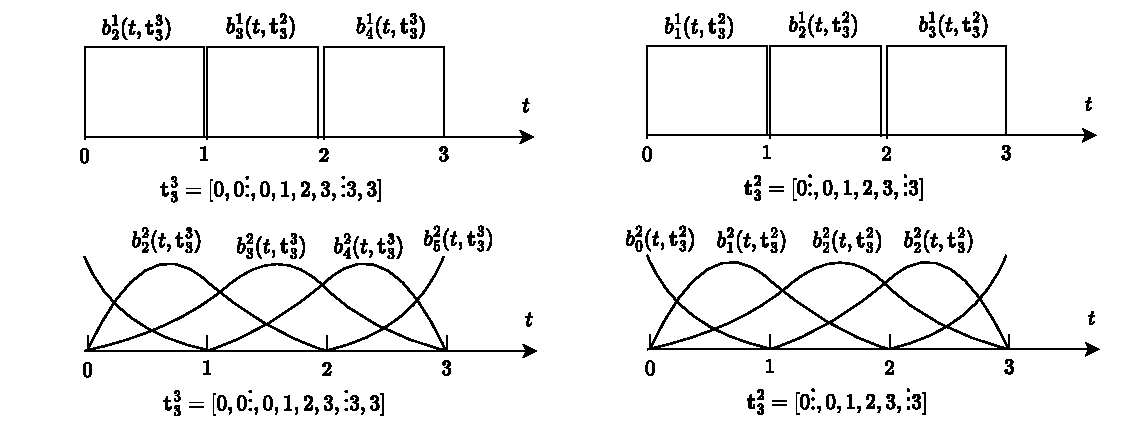
\includegraphics[width=0.99\textwidth]{./chap5_trajectory_planning/figures/shifting_property}
  \caption{Shifting property of uniform clamped B-spline basis functions.}
  \label{fig:shifting_property}  
\end{figure}
If on the other hand, the knot vector has one order lower, i.e., $\mathbf{t}_3^2 = [0\vdots, 0, 1, 2, 3, \vdots 3]$, then the basis vectors are also shown to the right in Figure~\ref{fig:shifting_property}.  It is clear that reducing the order of the knot vector by one, shifts the index of the basis vectors by one.  We can formalize these observations in the following lemma.
\begin{lemma} \label{lem:shifting_property}
For uniform or clamped uniform knot vectors $\mathbf{t}_M^k \in \mathbb{R}^{M+2k-1}$ and $\mathbf{t}_M^{k-1}\in\mathbb{R}^{M+2k-1}$ we have
\[
b_m^j(t; \mathbf{t}_M^k) = b_{m-1}^j(t; \mathbf{t}_M^{k-1}), \qquad j \leq k, \qquad m = 1, \dots, 2k+M.
\]	
Using vector notation we have that
\[
\underbrace{\bbf_M^{k-1}(t; \mathbf{t}_M^{k-1})}_{(M+k-1)\times 1} = S_{M+k} \underbrace{\bbf_M^{k-1}(t; \mathbf{t}_M^k)}_{(M+k)\times 1},
\]
where
\[
	S_{N} \defeq \begin{bmatrix} \mathbf{0}_{(N-1)\times 1}, & \mathbf{I}_{(N-1) \times (N-1)} \end{bmatrix}.
\]
\end{lemma}

We have the following lemma which gives the general formula for the derivative of the spline basis.
\begin{lemma}\label{lem:derivative_basis_functions}
If $\mathbf{t}$ is a general knot vector, then the $\ell^{th}$ derivative of the $k^{th}$ order spline function with  $0\leq \ell \leq k$, is given by
\[
\frac{d^\ell}{dt^\ell}b_m^k(t; \mathbf{t}) = k\left(\frac{\frac{d^{\ell-1}}{dt^{\ell-1}}b_m^{k-1}(t; \mathbf{t})}{\tau_{m+k}-\tau_m} - \frac{\frac{d^{\ell-1}}{dt^{\ell-1}}b_{m+1}^{k-1}(t; \mathbf{t})}{\tau_{m+k+1}-\tau_{m+1}} \right).
\]	
\end{lemma}
\marginnote{
The proof of Lemma~\ref{lem:derivative_basis_functions} is in~\cite{PieglTiller95}.
}

Using vector notation, we have the following formula for the derivative of a spline function.
\begin{lemma} \label{lem:derivative_of_spline}
Given the $k^{th}$-order uniform clamped spline function
\[
\mathbf{p}(t) = \Cbf \bbf_M^k(t), \quad t\in[0, M]
\]
we have that
\[
\frac{d\mathbf{p}}{dt}(t) = \Cbf D_M^k \bbf_M^{k-1}(t), \quad t\in[0, M]
\]	
where $D_M^k$ is the $(M+k)\times (M+k-1)$ derivative matrix given by
\begin{equation}\label{eq:D_k}
D_M^k = -\begin{bmatrix}\bar{D}_M^k \\ \mathbf{0}_{1\times(M+k-1)} \end{bmatrix} + \begin{bmatrix}\mathbf{0}_{1\times(M+k-1)} \\ \bar{D}_M^k \end{bmatrix},
\end{equation}
where
\begin{equation}\label{eq:D_k_bar}
\bar{D}_M^k = \text{diag}\left(\frac{k}{1}, \frac{k}{2}, \dots, \frac{k}{k-1}, \underbrace{1, \dots, 1}_{M-k+1}, \frac{k}{k-1}, \dots, \frac{k}{2}, \frac{k}{1}\right),
\end{equation}
is an $(M+k-1)\times(M+k-1)$ diagonal matrix.
\end{lemma}
\begin{proof}
Noting that
\[
\mathbf{p}(t) = \Cbf \bbf_M^k(t)
              = \sum_{m=0}^{M+k-2} \cbf_m b_m^k(t; \bar{\mathbf{t}}_M^k),
\]
we have that
\[
\frac{d\mathbf{p}}{dt} = \sum_{m=0}^{M+k-2} \cbf_m \frac{d b_m^k(t; \bar{\mathbf{t}}_M^k)}{dt}.
\]
From Lemma~\ref{lem:derivative_basis_functions} we get
\begin{align*}
\frac{d\mathbf{p}}{dt} &= \sum_{m=0}^{M+k-2} \cbf_m k\left(\frac{b_m^{k-1}(t; \bar{\mathbf{t}}_M^k)}{\tau_{m+k}-\tau_m} - \frac{b_{m+1}^{k-1}(t; \bar{\mathbf{t}}_M^k)}{\tau_{m+k+1}-\tau_{m+1}} \right) \\
&= \sum_{m=0}^{M+k-2} \cbf_m \left[ \left(\frac{k}{\tau_{m+k}-\tau_m}\right) b_m^{k-1}(t; \bar{\mathbf{t}}_M^k) - \left(\frac{k}{\tau_{m+k+1}-\tau_{m+1}}\right)  b_{m+1}^{k-1}(t; \bar{\mathbf{t}}_M^k) \right] \\
&= \left(\frac{k}{\tau_{k}-\tau_0}\right)\cbf_0 b_0^{k-1}(t; \bar{\mathbf{t}}_M^k) + \sum_{m=1}^{M+k-2} \left(\frac{k}{\tau_{m+k}-\tau_m}\right) \left(  \cbf_m - \cbf_{m-1}  \right) b_m^{k-1}(t; \bar{\mathbf{t}}_M^k) \\
&\qquad - \left(\frac{k}{\tau_{M+2k-1}-\tau_{M+k-1}}\right)\cbf_{M+k-2}b_{M+k-1}^{k-1}(t; \bar{\mathbf{t}}_M^k).
\end{align*}
Now note that since the first $k$ terms in the knot vector $\mathbf{t}_M^k$ are equal to zeros, and the last $k$ terms are equal to $M$, that $\tau_k-\tau_0 = \tau_{M+2k-1}-\tau_{M+k-1} = 0$, and therefore the first and last terms are zero.  Using the shifting property from Lemma~\ref{lem:shifting_property}, and changing the index by one, we get
\begin{equation}\label{eq:spline_deriviative_1}
\frac{d\mathbf{p}}{dt} = \sum_{m=0}^{M+k-3} \left(\frac{k}{\tau_{m+k}-\tau_{m}}\right) \left( \cbf_{m+1} - \cbf_{m}  \right) b_{m}^{k-1}(t; \mathbf{t}_M^{k-1}),
\end{equation}
where $\tau_\ast$ now corresponds to the knot vector 
\[
\mathbf{t}_M^{k-1} = [\underbrace{0, 0, \dots, 0}_{k-2}, 0, 1, 2, \dots, M, \underbrace{M, \dots, M}_{k-2}].
\]
From the definition of $\mathbf{t}_M^{k-1}$ we note that
\begin{align*}
& \frac{k}{\tau_{k}-\tau_0} = \frac{k}{1}, \quad
\frac{k}{\tau_{k+1}-\tau_1} = \frac{k}{2}, \quad
\dots \quad
\frac{k}{\tau_{2k-1}-\tau_{k-1}} = \frac{k}{k-1},  \\
&\frac{k}{\tau_{2k}-\tau_{k}} = \frac{k}{k}, \quad
\dots \quad
\frac{k}{\tau_{M+k-1} - \tau_{M-1}} = \frac{k}{k}, \\
& \frac{k}{\tau_{M+k} - \tau_{M}} = \frac{k}{k-1}, \quad
\dots \quad
\frac{k}{\tau_{M+2k-2} - \tau_{M+k-2}} = \frac{k}{1}
\end{align*}
Define the $(M+k-1)\times(M+k-1)$ diagonal matrix $\bar{D}_M^k$ in Equation~\eqref{eq:D_k_bar}, and the $(M+k)\times (M+k-1)$ derivative matrix $D_M^k$ in Equation~\eqref{eq:D_k},
then Equation~\eqref{eq:spline_deriviative_1} can be written as
\[
\frac{d\mathbf{p}}{dt} = \Cbf D_M^k \bbf_M^{k-1}(t).
\]
\end{proof}

From Lemma~\ref{lem:derivative_of_spline} we can derive a number of useful results, which we summarize in the corollary below.
\begin{corollary}
	Given the $k^{th}$-order uniform clamped B-spline function
	\[
	\mathbf{p}(t) = \Cbf \bbf_M^k(t), \quad t\in[0, M]
	\]
	we can make the following statements:
	\begin{description}
	\item[(i)] The derivative  $\frac{d\mathbf{p}}{dt}$ is a $(k-1)^{th}$-order uniform clamped B-spline function.
	\item[(ii)] The control points of $\frac{d\mathbf{p}}{dt}$ are given by
		\[
		C^{'} \defeq C D_M^k = \begin{pmatrix}
				\frac{k}{1} (\cbf_1 - \cbf_0)^\top \\
				\vdots \\
				\frac{k}{k-1} (\cbf_{k-1} - \cbf_{k-2})^\top \\
				(\cbf_k - \cbf_{k-1})^\top \\
				\vdots \\
				(\cbf_{M+1} - \cbf_{M})^\top \\
				\frac{k}{k-1} (\cbf_{M+2}-\cbf_{M+1})^\top \\
				\vdots \\
				\frac{k}{1} (\cbf_{M+k-1} - \cbf_{M+k-2})^\top
 				\end{pmatrix}^\top
 			\defeq \begin{pmatrix}
 			        \cbf_0^{'\top} \\
 			        \vdots \\
 			        \cbf_{M+k-2}^{'\top}
 				   \end{pmatrix}^\top.
		\]
	\item[(iii)] The $\ell^{th}$ derivative of $\mathbf{p}(t)$ for $0\leq\ell\leq k-1$ is given by
		\begin{align*}
			\frac{d^{\ell}\mathbf{p}}{dt^{\ell}} 
			&= C D_M^k D_M^{k-1} \dots D_M^{k-\ell+1} \bbf_M^{k-\ell}(t), \quad t\in [0, M] \\
			&= C^{(\ell)} \bbf_M^{k-\ell}(t), \quad t\in [0, M] \\
			&= C \boldsymbol{\psi}^{(\ell)}(t), \quad t\in [0, M] \\
		\end{align*}
		where the control points of the $(k-\ell)^{th}$ order spline are given by
		\[
			C^{(\ell)} = C D_M^k D_M^{k-1} \dots D_M^{k-\ell+1}
		\]
		or alternatively, the $\ell^{th}$ derivative of the basis vector $\bbf_M^k(t)$ is given by
		\[
			\boldsymbol{\psi}^{(\ell)} \defeq \frac{d^{\ell}\bbf_M^k(t)}{dt^{\ell}} = D_M^k D_M^{k-1} \dots D_M^{k-\ell+1} \bbf_M^{k-\ell}(t), \quad t\in [0, M].
		\]
	\item[(iv)] The derivative of $\mathbf{p}(t)$ at $t=0$ is given by the difference of the first two control points as
		\[
			\frac{d\mathbf{p}}{dt}(0) = k(\cbf_1 - \cbf_0).
		\]
	\item[(v)] The derivative of $\mathbf{p}(t)$ at $t=M$ is given by the difference of the last two control points as
		\[
			\frac{d\mathbf{p}}{dt}(M) = k(\cbf_{M+k-1} - \cbf_{M+k-2}).
		\]
	\item[(vi)] If the desired B-spline trajectory with $k\geq 3$ has the following desired endpoint conditions:
		\begin{align*}
			\text{Initial position:} &\quad \mathbf{p}(0) \stackrel{des}{=} \mathbf{p}_0 \\	
			\text{Final position:} &\quad \mathbf{p}(M) \stackrel{des}{=} \mathbf{p}_f \\
			\text{Initial velocity:} &\quad \frac{d\mathbf{p}}{dt}(0) \stackrel{des}{=} \mathbf{v}_0 \\	
			\text{Final velocity:} &\quad \frac{d\mathbf{p}}{dt}(M) \stackrel{des}{=} \mathbf{v}_f, \\
			\text{Initial acceleration:} &\quad \frac{d^2\mathbf{p}}{dt^2}(0) \stackrel{des}{=} \mathbf{a}_0 \\	
			\text{Final acceleration:} &\quad \frac{d^2\mathbf{p}}{dt^2}(M) \stackrel{des}{=} \mathbf{a}_f,
		\end{align*}
		then the first and last three control points satisfy
		\begin{align*}
			\cbf_0 &= \mathbf{p}_0 \\
			\cbf_1 &= \mathbf{p}_0 + \frac{1}{k} \mathbf{v}_0 \\
			\cbf_2 &= \mathbf{p}_0 + \frac{3}{k} \mathbf{v}_0 + \frac{2}{k(k-1)}\mathbf{a}_0 \\
			\cbf_{M+k-3} &= \mathbf{p}_f - \frac{3}{k}\mathbf{v}_f + \frac{2}{k(k-1)}\mathbf{a}_f \\
			\cbf_{M+k-2} &= \mathbf{p}_f - \frac{1}{k}\mathbf{v}_f \\
			\cbf_{M+k-1} &= \mathbf{p}_f.
		\end{align*}
	\end{description}
\end{corollary}



%---------------------------------------------------------------
\subsection{B-Spline Planning for Chains of Integrators}

%---------------------------------------------------------------
\subsection{B-Splines on Lie Groups}

%---------------------------------------------------------------
\subsection{B-Splines Surfaces}

Suppose that the objective is to create a one dimensional surface over a two dimensional domain.  For example, a terrain map is a one dimensional surface of altitudes over the north-east plane.  In this section we will explore the use of B-splines to accomplish this objective. Many of the ideas and notation in this section come from~\cite{RodriguesTsiogkasAguiar20}.

If $\mathbf{t}_M^k$ and $\mathbf{t}_N^k$ are two different $k^{th}$ order uniform clamped knot vectors of length $M$ and $N$ understood to define knots in the $x$ and $y$ directions, then following Equation~\eqref{eq:clamped_uniform_spline}, a clamped uniform B-spline surface is defined as 
\begin{equation}\label{eq:spline_surface1}
S(x, y) \defeq \sum_{m=0}^{M+k-1} \sum_{n=0}^{N+k-1} c_{m,n} b^k_m(x; \mathbf{t}_M^k) b^k_n(y; \mathbf{t}_N^k), \quad x\in[0,M], y\in[0, N],
\end{equation}
where $c_{m, n}$, $m=0, \dots, M+k-1$, $n=0, \dots, N+k-1$ are the control points of the surface.  Defining the matrix $\Cbf=\{c_{m,n}\}$, and defining the spatial variable $\sbf = (s_1, s_2)^\top$, we can write Equation~\eqref{eq:spline_surface1} as
\begin{equation}\label{eq:spline_surface2}
S(\sbf) = \bbf^k_M(s_1)^\top \Cbf \bbf^k_N(s_2), \quad \sbf\in[0, M]\times[0, N],
\end{equation}
This equation is linear in the spline coefficients $\Cbf$.  In other words, if $S_1(\sbf)=\bbf^k_M(s_1)^\top \Cbf_1 \bbf^k_N(s_2)$, and $S_1(\sbf)=\bbf^k_M(s_1)^\top \Cbf_2 \bbf^k_N(s_2)$ are two different spline surfaces, then 
\[
S(\sbf)\defeq \alpha S_1(\sbf) + \beta S_2(\sbf) = \bbf^k_M(s_1)^\top \left(\alpha\Cbf_1 + \beta\Cbf_2\right) \bbf^k_N(s_2),
\]
is also a spline surface.

Suppose that instead of defining the surface over the set $[0, M]\times[0, N]$ we instead would like to define the surface over the set $[\underline{X}, \overline{X}]\times[\underline{Y}, \overline{Y}]$.  Given the shift and scaling properties is Lemmas~\ref{lem:basis_are_shift_invariant} and~\ref{lem:bases_are_scale_invariant} we have 
\begin{equation}\label{eq:spline_surface3}
S(\sbf) = \bbf^k_M\left(\frac{M(s_1-\underline{X})}{\overline{X}-\underline{X}}\right)^\top \Cbf \bbf^k_N\left(\frac{N(s_2-\underline{Y})}{\overline{Y}-\underline{Y}}\right), \quad \sbf\in[\underline{X}, \overline{X}]\times[\underline{Y}, \overline{Y}].
\end{equation}

\begin{figure}[hbt]
  \centering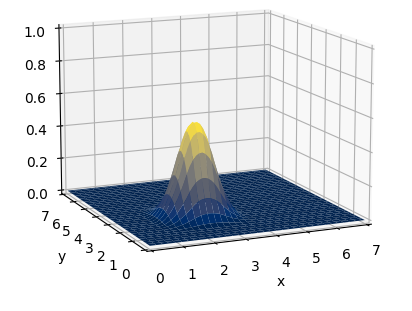
\includegraphics[width=0.9\textwidth]{./chap5_trajectory_planning/figures/spline_surface_basis}
  \caption{A single second order spline bases function $b_3^2(s_1)b_3^2(s_2)$.}
  \label{fig:spline_surface_bases}  
\end{figure}


%
%The basic idea is to create two-dimensional bases vectors as the tensor product of the one-dimensional bases vectors introduced in Section~\ref{sec:b-spline-basis-functions}.  For example, replacing the time variable $t$ with the spacial variables $x$ and $y$, the $k^{th}$-order two dimensional basis vectors are defined as
%\[
%b^k_{m,n}(x,y) = b^k_m(x; \mathbf{t}_1) b^k_n(y; \mathbf{t}_2), 
%\]
%where $T=\mathbf{t}_1 \times \mathbf{t}_2$ is the two-dimensional knot array, and $b^{k}_m(x; \mathbf{t}_1)$ is the $k^{th}$-order spline function with index $m$ and knot vector $\mathbf{t}_1$, and similarly for $b^k_n(y; \mathbf{t}_2)$.
%
%
%If $\mathbf{t}_M^k$ and $\sbf_N^k$ are $k^{th}$ order uniform clamped knot vectors of length $M$ and $N$, then 
%$\mathbf{T}^k_{M,N}\defeq \mathbf{t}_M^k \times \sbf_M^k$ is a $k^{th}$ order uniform clamped knot array of size (M,N).  For example, if $\mathbf{t}_3^2 = [0, 0, 0, 1, 2, 3, 3, 3]$, and $\sbf_2^2 = [0, 0, 0, 1, 2, 2, 2]$, then
%\[
%\mathbf{T}^2_{3,2} = \begin{bmatrix} 
%						(0, 0) & (0, 0) & (0, 0) & (0, 1) & (0, 2) & (0, 2) & (0, 2) \\
%						(0, 0) & (0, 0) & (0, 0) & (0, 1) & (0, 2) & (0, 2) & (0, 2) \\
%						(0, 0) & (0, 0) & (0, 0) & (0, 1) & (0, 2) & (0, 2) & (0, 2) \\
%						(1, 0) & (1, 0) & (1, 0) & (1, 1) & (1, 2) & (1, 2) & (1, 2) \\
%						(2, 0) & (2, 0) & (2, 0) & (2, 1) & (2, 2) & (2, 2) & (2, 2) \\
%						(3, 0) & (3, 0) & (3, 0) & (3, 1) & (2, 2) & (3, 2) & (3, 2) \\
%						(3, 0) & (3, 0) & (3, 0) & (3, 1) & (2, 2) & (3, 2) & (3, 2) \\
%						(3, 0) & (3, 0) & (3, 0) & (3, 1) & (2, 2) & (3, 2) & (3, 2)
% 					 \end{bmatrix}.
%\]
%
%
%Recall that if $\mathbf{A}$ is an $m\times n$ matrix and $\bbf$ is $p\times q$ matrix, then the Kronecker product of $\mathbf{A}$ and $\bbf$ is defined as 
%\[
%\mathbf{A}\otimes\bbf \circeq \begin{pmatrix} 
% 										a_{11}B & a_{12}B & \dots & a_{1n}B \\	
% 										a_{21}B & a_{22}B & \dots & a_{2n}B \\
% 										\vdots & \vdots & \dots & \vdots \\
% 										a_{m1}B & a_{m2}B & \dots & a_{mn}B \\	
% 									\end{pmatrix}.
%\]
%We will use the Kronecker product to simplify the notation associated with spline surfaces.  Let $\xbf=(x_1, x_2)^\top\in\mathbb{R}^2$, and let $\bbf^k_M(x_1; \mathbf{t}_M^k)$ and $\bbf^k_N(x_2; \sbf_N^k$ be $k^{th}$ order basis vectors as defined in Equation~\eqref{eq:basis_vector} and $T^k_{M,N}=\mathbf{t}_M^k \times \sbf_N^k$, then define the basis vector 
%\[
%\bbf^k_{M,N}(\xbf; T^k_{M,N}) = \bbf^k_M(x_1; \mathbf{t}_M^k) \otimes \bbf^k_N(x_2; \sbf_N^k), 
%\]
%where we will drop to inclusion of the knot array and write simply $\bbf^k_{M,N}(\xbf)\circeq\bbf^k_{M,N}(\xbf; T^k_{M,N})$.
%Similarly, defining the control vector 
%\[
%\cbf \circeq \begin{pmatrix} c_{1,1} & c_{1,2} & \dots & c_{1,N} & \dots & c{M,1} & \dots & c_{M,N} \end{pmatrix}^\top,
%\]
%we get that
%\[
%S^k(\xbf) = \cbf^\top  \bbf^k_{M,N}(\xbf), \qquad \xbf \in [0,M]\times[0,N].
%\]

The Python code below plots a randomly defined terrain map over the domain $[-\pi, \pi]\times[-2\pi, 2\pi]$.
\begin{lstlisting}
import numpy as np
import splipy as sp
import matplotlib.pyplot as plt
from bspline_tools import uniform_clamped_knots

def draw_random_surface(order=2, M=10, N=10,
                        Xmin=-3.14159, Xmax=3.14159,
                        Ymin=-2*3.14159, Ymax=2*3.14159):
    # define the spline surface
    knots_x = uniform_clamped_knots(k=order, M=M)
    knots_y = uniform_clamped_knots(k=order, M=N)
    basis_x = sp.BSplineBasis(order + 1, knots_x)
    basis_y = sp.BSplineBasis(order + 1, knots_y)
    C = np.random.rand(M + order, N + order)  # random control points
    surface = sp.Surface(basis_x, basis_y,
                         np.reshape(C, ((M + order) * (N + order), 1)))
    # plot the spline surface
    x = np.linspace(Xmin, Xmax, 10 * M)
    y = np.linspace(Ymin, Ymax, 10 * N)
    S = surface(M*(x-Xmin)/(Xmax-Xmin),
                N*(y-Ymin)/(Ymax-Ymin))  # surface points
    fig = plt.figure()
    ax = fig.add_subplot(111, projection='3d')
    plt.xlabel('x')
    plt.ylabel('y')
    x_pts, y_pts = np.meshgrid(x, y)  # grid points
    ax.plot_surface(x_pts, y_pts, S[:, :, 0])
    plt.show()
\end{lstlisting}
The result of running this code is shown in Figure~\ref{fig:random_spline_surface}
\begin{figure}[hbt]
  \centering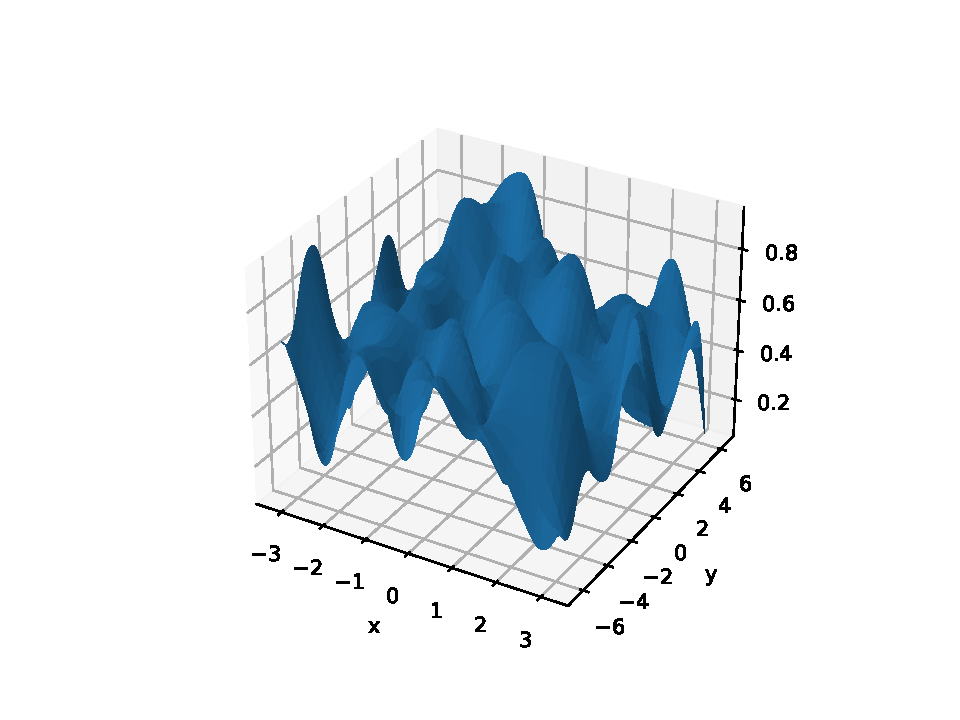
\includegraphics[width=0.9\textwidth]{./chap5_trajectory_planning/figures/random_spline_surface}
  \caption{Spline surface with randomly generated control points.}
  \label{fig:random_spline_surface}  
\end{figure}





%---------------------------------------------------------------
\subsection{B-Splines and Occupancy Maps}

Since B-spline surfaces are continuous the spatial variable $\sbf\in\mathbf{R}^2$, the occupancy map will also be continuous (as opposed to an occupancy grid).  Following~\cite{RodriguesTsiogkasAguiar20}, at every point $\sbf$ we can define the discrete random variable $m(\sbf)$ to be the occupancy of the map, where $m(\sbf)=1$ indicates that a target is located at $\sbf$, and $m(\sbf)=0$ indicates that a target is not located at $\sbf$.  
%
Similarly, define the discrete random variable $z(\sbf)$ to be the measurement state, where $z(\sbf)=1$ indicates that a target is detected at $\sbf$, and $z(\sbf)=0$ indicates that a target is not detected at $\sbf$.
% 
Let $\xbf_t$ be the state of the UAV at time $t$, where the UAV state evolution equations are given by
\[
\xbf_t = f(\xbf_{t-1}, \ubf_{t-1}) + \eta_t
\]
where $\eta_t\sim\mathcal{N}(0, Q)$. Let $\fov{\xbf_t}$ be the area on the terrain what is seen by the camera when the state is $\xbf_t$, then the measurement model is given by
%
\begin{align}
	p(z(\sbf)=1 \mid m(\sbf)=1, \xbf) &= \begin{cases}
 											p_d &\quad \mathbf{s}\in\fov{\xbf} \\
 											0 &\quad \text{otherwise}
 										 \end{cases} 
	\label{eq:prob_z=1:m=1}\\
	p(z(\sbf)=0 \mid m(\sbf)=1, \xbf) &= \begin{cases}
 											1-p_d &\quad \mathbf{s}\in\fov{\xbf} \\
 											1 &\quad \text{otherwise}
 										 \end{cases}
	\label{eq:prob_z=0:m=1}\\
	p(z(\sbf)=1 \mid m(\sbf)=0, \xbf) &= \begin{cases}
 											p_f &\quad \mathbf{s}\in\fov{\xbf} \\
 											1 &\quad \text{otherwise}
 										  \end{cases}
	\label{eq:prob_z=1:m=0}\\
	p(z(\sbf)=0 \mid m(\sbf)=0, \xbf) &= \begin{cases}
 											1-p_f &\quad \mathbf{s}\in\fov{\xbf} \\
 											0 &\quad \text{otherwise}
 										  \end{cases},
 	\label{eq:prob_z=1:m=0}
\end{align}
where $p_d$ is the probability of detection, and $p_f$ is the probability of false alarm.

Let $Z_t(\sbf) = \{z_t(\sbf), z_{t-1}(\sbf), \dots, z_0(\sbf)\}$ be the set of measurements of map location $\sbf$ over the time horizon $[0, t]$.  Using Bayes's law we have
\begin{align*}
	p(m(\sbf)=1 \mid Z_t(\sbf)) &= \frac{p(z_t(\sbf)\mid m(\sbf)=1, Z_{t-1}(\sbf)) p(m(\sbf)=1 \mid Z_{t-1}(\sbf))}{p(z_t(\sbf) \mid Z_{t-1}(\sbf))} \\
	p(m(\sbf)=0 \mid Z_t(\sbf)) &= \frac{p(z_t(\sbf)\mid m(\sbf)=0, Z_{t-1}(\sbf)) p(m(\sbf)=0 \mid Z_{t-1}(\sbf))}{p(z_t(\sbf) \mid Z_{t-1}(\sbf))}
\end{align*}
Defining the odds of a discrete random variable as
\[
\odd{x} \defeq \frac{p(x=1)}{p(x=0)},
\]
we get that 
\begin{align*}
	\odd{m(\sbf)\mid Z_t(\sbf), \xbf_t} &= \frac{p(m(\sbf)=1 \mid Z_t(\sbf), \xbf_t)}{p(m(\sbf)=0 \mid Z_t(\sbf), \xbf_t)} \\
	&= \frac{p(z_t(\sbf) \mid m(\sbf)=1, Z_{t-1}(\sbf), \xbf_t) \, p(m(\sbf)=1)\mid Z_{t-1}(\sbf), \xbf_t)}{p(z_t(\sbf)\mid m(\sbf)=0, Z_{t-1}(\sbf), \xbf_t) \, p(m(\sbf)=0)\mid Z_{t-1}(\sbf), \xbf_t)} \\
	&= \odd{m(\sbf) \mid Z_{t-1}(\sbf), \xbf_t}  \frac{p(z_t(\sbf)\mid m(\sbf)=1, Z_{t-1}(\sbf), \xbf_t)}{p(z_t(\sbf)\mid m(\sbf)=0, Z_{t-1}(\sbf), \xbf_t)}.
\end{align*}
Assuming that the current measurement is conditionally independent of previous measurements we get
\begin{align*}
	\odd{m(\sbf)\mid Z_t(\sbf), \xbf_t} 
		&= \odd{m(\sbf) \mid Z_{t-1}(\sbf), \xbf_t}  \frac{p(z_t(\sbf)\mid m(\sbf)=1, \xbf_t)}{p(z_t(\sbf)\mid m(\sbf)=0, \xbf_t)}.
\end{align*}
Taking the natural logarithm of each side gives
\[
\log\odd{m(\sbf)\mid Z_t(\sbf), \xbf_t} = \log \odd{m(\sbf) \mid Z_{t-1}(\sbf), \xbf_t} + \log\left(\frac{p(z_t(\sbf)\mid m(\sbf)=1, \xbf_t)}{p(z_t(\sbf)\mid m(\sbf)=0, \xbf_t)}\right).
\]
Defining the expected value (over random variable $\xbf_t$) as
\[
S_t(\sbf) \defeq E\{\log\odd{m(\sbf)\mid Z_t(\sbf), \xbf_t}\},
\]
then the expected log-odds surface at time $t$ is given by
\[
S_t(\sbf) = S_{t-1}(\sbf) + \int\log\left[ \frac{p(z_t(\sbf)\mid m(\sbf)=1, \xbf_t)}{p(z_t(\sbf)\mid m(\sbf)=0, \xbf_t)}\right]p(\xbf_t)d\xbf_t.
\] 

Defining the measurement function as 
\begin{equation} \label{eq:measurement_function}
U(z_t(\sbf), \sbf) \defeq \int\log\left[ \frac{p(z_t(\sbf)\mid m(\sbf)=1, \xbf_t)}{p(z_t(\sbf)\mid m(\sbf)=0, \xbf_t)}\right]p(\xbf_t)d\xbf_t,	
\end{equation}
then the log-odds update expression is
\begin{equation}\label{eq:log_odds_surface_update}
S_t(\sbf) = S_{t-1}(\sbf) + U(z_t(\sbf), \sbf).
\end{equation}

Following~\cite{RodriguesTsiogkasAguiar20} we will represent $S_t(\sbf)$ using a B-spline surface as 
\begin{equation}\label{eq:log_odds_surface}
S_t(\sbf) = \bbf_M^k(s_1)^\top C_t \bbf_N^k(s_2), \quad \sbf \in [0,M]\times[0,N].
\end{equation}
The probability that the target is located at $\sbf$ can be recovered from $S_t(\sbf)$ using the formula
\[
p(m(\sbf)=1\mid Z_t(\sbf)) = \frac{e^{S_t(\sbf)}}{1+e^{S_t(\sbf)}}.
\]

\begin{lemma}\label{lem:measurement_update_equation}
	Given the log-odds spline surface~\eqref{eq:log_odds_surface}, a measurement function $U(z_t(\sbf), \sbf)$, and the log-odds update equation~\eqref{eq:log_odds_surface_update}, the optimal update for the spline coefficients after a measurement at $\sbf \in [0,M]\times[0,N]$ is given by
	\begin{equation}\label{eq:coefficient_update_3}
	\Cbf_t = \Cbf_{t-1} + \mathbf{B}_{M,N}^k(\sbf) U(z_t(\sbf), \sbf), 
	\end{equation}
	where
	\begin{equation}\label{eq:measurement_update_matrix_B}
	\mathbf{B}_{M,N}^k(\sbf) \defeq \frac{\bbf_M^k(s_1)\bbf_N^k(s_2)^\top}{\norm{\bbf_M^k(s_1)}^2\norm{\bbf_N^k(s_2)}^2}
	\end{equation}
\end{lemma}
\begin{proof}
The proof follows the discussion given in~\cite{RodriguesTsiogkasAguiar20}.
%
Define the $\vec{\cdot}$ operation on a matrix to be the operation of stacking all of the columns of a matrix into a single vector, i.e., $\vec{(\cbf_1, \dots, \cbf_N)}=(\cbf_1^\top, \dots, \cbf_N^\top)^\top$, and let $\otimes$ denote the Kronecker product. As shown in~\cite{Kronecker_vect}, if $A$, $X$, and $B$ are compatible matrices, then $\vec{AXB}=(B^\top \otimes A)\vec{X}$.  Accordingly, we can write the spline surface~\eqref{eq:log_odds_surface} as
\begin{align*}
S_t(\sbf) &= \bbf_M^k(s_1)^\top \Cbf_t \bbf_N^k(s_2) \\
		  &= \vec{\bbf_M^k(s_1)^\top \Cbf_t \bbf_N^k(s_2)} \\
		  &= \left[\bbf_N^k(s_2)^\top \otimes \bbf_M^k(s_1)^\top \right] \vec{\Cbf_t} \\
		  &= \phibf(\sbf)^\top \cbf_t,
\end{align*}
where $\phibf(\sbf)\defeq \bbf_N^k(s_2) \otimes \bbf_M^k(s_1)$, and $\cbf_t \defeq \vec{\Cbf_t}$.

Consider the log-odds update Equation~\eqref{eq:log_odds_surface_update}, define the error equation at $\sbf$ to be
\begin{equation}\label{eq:error_log_odds}
e(\cbf_t) \defeq \phibf(\sbf)^\top \cbf_t - \phibf(\sbf)^\top \cbf_{t-1} - U(z_t(\sbf), \sbf),
\end{equation}
and consider the cost function $J(\cbf_t)=\frac{1}{2}e(\cbf_t)^2$.  Using a gradient descent update law for $\cbf_t$ would result in
\begin{align*}
\cbf_t &= \cbf_{t-1} - \mu \frac{\partial J}{\partial\cbf_t} \\
       &= \cbf_{t-1} - \mu \frac{\partial e}{\partial\cbf_t} e(\cbf_t) \\
	   &= \cbf_{t-1} - \mu \phibf(\sbf) e(\cbf_t) \\
	   &= \cbf_{t-1} - \mu \phibf(\sbf) \left(\phibf(\sbf)^\top \cbf_t - \phibf(\sbf)^\top \cbf_{t-1} - U(z_t(\sbf), \sbf)\right).
\end{align*}
Solving for $\cbf_t$ gives 
\begin{equation}\label{eq:coefficient_update_1}
\cbf_t = \cbf_{t-1} + \mu \left[I + \mu \phibf(\sbf)\phibf(\sbf)^\top\right]^{-1}\phibf(\sbf) U(z_t(\sbf), \sbf),
\end{equation}
where we note that $\left[I + \mu \phibf(\sbf)\phibf(\sbf)^\top\right]$ is invertible for all $\mu>0$ since $\phibf\phibf^\top$ is positive semi-definite.  From the matrix inversion lemma we have that
\[
\left[I + \mu \phibf(\sbf)\phibf(\sbf)^\top\right]^{-1} = I - \mu\frac{\phibf(\sbf)\phibf(\sbf)^\top}{1+\mu\norm{\phibf(\sbf)}^2}.
\]
Therefore Equation~\eqref{eq:coefficient_update_1} becomes
\begin{align}
	\cbf_t &= \cbf_{t-1} + \mu \left[I - \mu\frac{\phibf(\sbf)\phibf(\sbf)^\top}{1+\mu\norm{\phibf(\sbf)}^2}\right]\phibf(\sbf)		   U(z_t(\sbf), \sbf) \notag \\
	       &= \cbf_{t-1} + \mu \phibf(\sbf)\left[1 - \mu\frac{\norm{\phibf(\sbf)}^2}{1+\mu\norm{\phibf(\sbf)}^2}\right]U(z_t(\sbf), \sbf) \notag \\
	       &= \cbf_{t-1} + \left[\frac{\mu}{1+\mu\norm{\phibf(\sbf)}^2}\right]\phibf(\sbf) U(z_t(\sbf), \sbf).
	       \label{eq:coefficient_update_2}
\end{align}
The error equation~\eqref{eq:error_log_odds} then becomes
\[
e(\cbf_t) = \left[\frac{\mu\norm{\phibf(\sbf)}^2}{1+\mu\norm{\phibf(\sbf)}^2}\right] U(z_t(\sbf), \sbf) - U(z_t(\sbf), \sbf).
\]
Therefore, the squared error is minimized in the limit as $\mu\to\infty$.  As $\mu\to\infty$, the spline coefficient update equation~\eqref{eq:coefficient_update_2} becomes
\[
\cbf_t = \cbf_{t-1} + \frac{\phibf(\sbf)}{\norm{\phibf(\sbf)}^2} U(z_t(\sbf), \sbf),
\]
or in other words
\[
\vec{\Cbf_t} = \vec{\Cbf_{t-1}} + \frac{\bbf_N^k(s_2) \otimes \bbf_M^k(s_1)}{\norm{\bbf_N^k(s_2) \otimes \bbf_M^k(s_1)}^2} U(z_t(\sbf), \sbf).
\]
Unstacking the vectors into matrices, and noting that 
\[
\bbf_N^k(s_2) \otimes \bbf_M^k(s_1)=\vec{\bbf_M^k(s_1)\bbf_N^k(s_2)^\top}
\]
and that 
\[
\norm{\bbf_N^k(s_2) \otimes \bbf_M^k(s_1)}^2=\norm{\bbf_M^k(s_1)}^2 \norm{\bbf_N^k(s_2)}^2,
\] 
results in Equation~\eqref{eq:coefficient_update_3}.
\end{proof}

\begin{lemma} \label{lem:B_is_sparse}
Let $\mathbf{B}_{M,N}^k(\sbf)$
be the $(M+k)\times(N+k)$ measurement update matrix defined in Equation~\eqref{eq:measurement_update_matrix_B}.  
If $\sbf \in [m, m+1]\times[n, n+1] \subset [0, M]\times[0,N]$, then the only nonzero elements of $\mathbf{B}_{M,N}^k(\sbf)$ is the $(k+1)\times(k+1)$ sub-matrix with upper-left index equal to $[m,n]$.
\end{lemma}
\begin{proof}
The proof follows directly from Lemma~\ref{lem:finite_num_control_points}.	
\end{proof}

Lemma's~\ref{lem:measurement_update_equation} and~\ref{lem:B_is_sparse} taken together imply that every measurement $U(z_t(\sbf), \sbf)$ only requires the update of $(k+1)^2$ spline coefficients, and is therefore, extremely computationally efficient.  For example, if the order of the splines is $k=3$, then the measurement update is over a $4\times 4$ submatrix, independent of the size of $M$ and $N$, which for large worlds could be in tens of thousands.  This property has obvious implications for cooperative control where vehicles can build cooperative maps with limited communication.  


We now turn our attention to the computation of the update equation $U(z_t(\sbf), \sbf)$ given by Equation~\eqref{eq:measurement_function} as
\[
U(z_t(\sbf), \sbf) = \int_{\xibf\in\mathbb{R}^n}\log\left[ \frac{p(z_t(\sbf)\mid m(\sbf)=1, \xbf_t)}{p(z_t(\sbf)\mid m(\sbf)=0, \xbf_t)}\right]p_{X_t}(\xibf)d\xibf,
\]
where 
\[
p_{X_t}(\xibf) \defeq \frac{1}{\sqrt{2\pi^n|P_t|}}exp\left(\frac{1}{2}(\xibf-\xbf_t)^\top \Pbf_t^{-1} (\xibf-\xbf_t)\right)
\]
is the posterior probability density associated with state estimate of the aircraft, where $(\xbf_t, \Pbf_t)$ are the mean and covariance given by, for example, an extended Kalman filter.
From Equations~\eqref{eq:prob_z=1:m=1}--\eqref{eq:prob_z=1:m=0} we get that 
\[
\log\left[ \frac{p(z_t(\sbf)\mid m(\sbf)=1, \xbf_t)}{p(z_t(\sbf)\mid m(\sbf)=0, \xbf_t)}\right] 
	= \begin{cases}
 		\log\left(\frac{p_d}{p_f}\right), &\quad z_t(\sbf)=1 \text{~and~} \sbf\in\fov{\xbf_t} \\
 		\log\left(\frac{1-p_d}{1-p_f}\right), &\quad z_t(\sbf)=0 \text{~and~} \sbf\in\fov{\xbf_t} \\
 		? &\quad \sbf\not\in\fov{\xbf_t}
 	  \end{cases}.
\]
Defining the set $\fovinv{\sbf}\defeq\{\xibf\in\mathbb{R}^n: \sbf\in\fov{\xibf}\}$ and defining 
\begin{equation}\label{eq:Ubar}
\bar{U}(\sbf) \defeq \int_{\xibf\in\fovinv{\sbf}} p_{X_t}(\xibf)d\xibf
\end{equation}
we get that the measurement update equation is given by
\[
U(z_t(\sbf), \sbf) = 
	\begin{cases}
 		\bar{U}(\sbf)\log\left(\frac{p_d}{p_f}\right), &\quad z_t(\sbf)=1 \\
 		\bar{U}(\sbf)\log\left(\frac{1-p_d}{1-p_f}\right), &\quad z_t(\sbf)=0
 	  \end{cases}.
\]

The computation of $\bar{U}(\sbf)$ will require a few assumptions, as well as numerical approximation of the integral.
In approximating Equation~\eqref{eq:Ubar} we will assume that the field of view of the camera is rectangular with field-of-view angles $\eta_x$, and $\eta_y$ in the $x$ and $y$ axes of the camera frame. 
%
\begin{figure}[hbt]
  \centering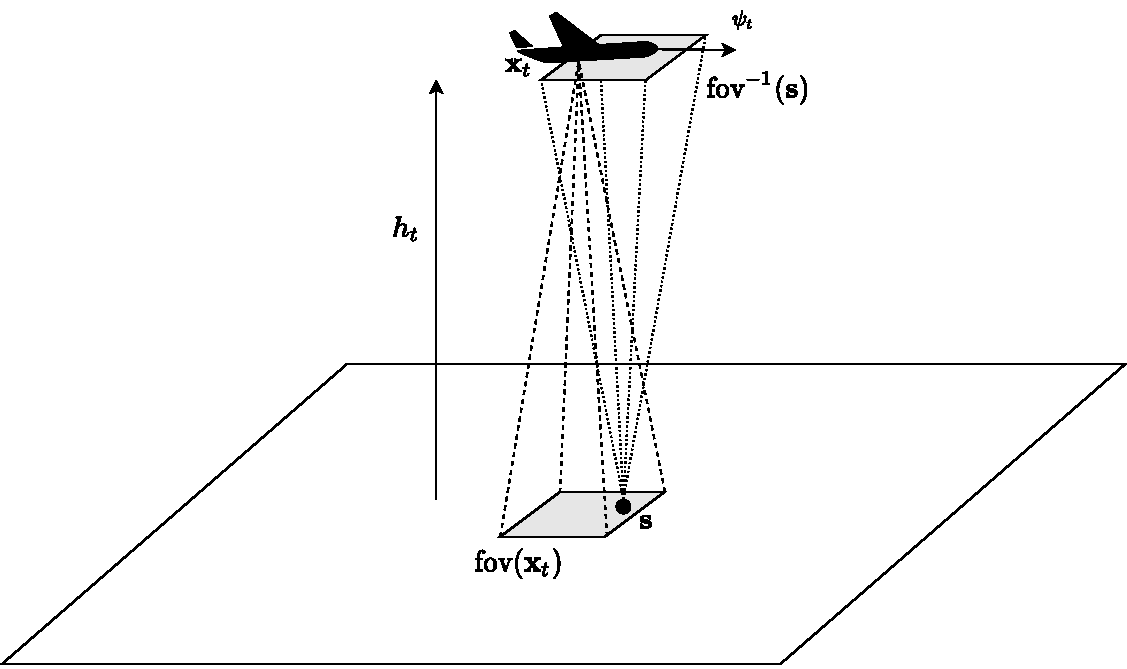
\includegraphics[width=0.99\textwidth]{./chap5_trajectory_planning/figures/inverse_field_of_view}
  \caption{Field-of-view of the camera given $\xbf_t$, and inverse field-of-view of the camera given $\sbf$.}
  \label{fig:inverse_field_of_view}  
\end{figure}
%
Figure~\ref{fig:inverse_field_of_view} shows the physical geometry.  We will assume that the camera is gimbaled to point toward the center of the earth, and that the ground is approximately flat.  In that case, the physical footprint of the camera field of view will also be rectangular with physical dimensions given by $M_x = 2h\tan(\eta_x/2)$ and $M_y=2h\tan(\eta_y/2)$, where $h=-p_d$ is the altitude of the aircraft.  For the purposes of this section, we will assume that there is uncertainty in the north-east position of the aircraft, but that the altitude and attitude are known.  If the aircraft is equipped with an altimeter and digital compass, then this is a reasonable assumption.  
Given the estimated state of the UAV $\xbf_t$ we can determine footprint of field-of-view on the ground.  We assume that the target detection software can detect targets to some resolution in the camera, and divide the field of view into rectangular bins accordingly.  Define $N_x$ and $N_y$ so that there are $2N_x+1$ bins in the $x$-direction, and $2N_y+1$ bins in the $y$-direction, as shown in Figure~\ref{fig:riemann_sum}.  We define the number of bins in this way to ensure an odd number in each direction. 
\begin{figure}[hbt]
  \centering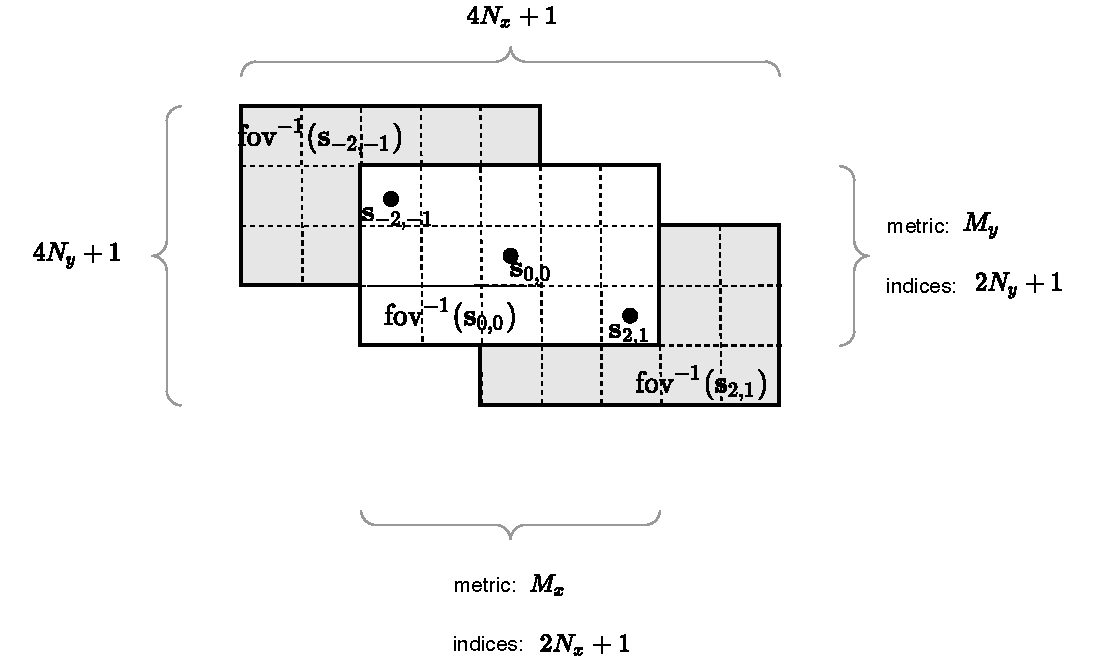
\includegraphics[width=0.99\textwidth]{./chap5_trajectory_planning/figures/riemann_sum}
  \caption{Riemann sum over camera field-of-view.}
  \label{fig:riemann_sum}  
\end{figure}
The physical size of each bin is given by
\[
	A = \left(\frac{M_x}{2N_x+1}\right)\left(\frac{M_y}{2N_y+1}\right)
	  = \left(\frac{2h\tan(\eta_x/2)}{2N_x+1}\right)\left(\frac{2h\tan(\eta_y/2)}{2N_y+1}\right).
\]

Suppose that the state of the UAV at time $t$ is given by
\[
\xbf_t = (p_n, p_e, p_d, v_n, v_e, v_d, \phi, \theta, \psi)^\top
\]
then the position of the center of the $(i,j)^{th}$ bin is given by
\[
\sbf_{i,j} = \begin{pmatrix} p_n \\ p_e \end{pmatrix} + \begin{pmatrix} 0 & -1 \\ 1 & 0 \end{pmatrix} \begin{pmatrix}\cos\psi & \sin\psi \\ -\sin\psi & \cos\psi \end{pmatrix}\begin{pmatrix} \frac{M_x(h)}{2N_x+1} i \\ \frac{M_y(h)}{2N_y+1} j \end{pmatrix}, 
\]
for $i=-N_x, \dots, N_x$ and $j=-N_y, \dots, N_y$.  

Given a camera measurement, we will need to update the log-odds spline map for each $\sbf_{i,j}$ in the camera field of view. To compute $\bar{U}(\sbf_{i,j})$ requires the inverse field-of-view of $\sbf_{i,j}$.  Under the assumption that the $h$ and $\psi$ are known, the inverse field-of-view will a rectangle on the altitude plane of the aircraft centered at $\sbf_{i,j}$ as shown in Figure~\ref{fig:inverse_field_of_view}.  Using a similar binning notation for the inverse field-of-view, the north-east coordinates of the center of the $(m,n)^{th}$ bin of the inverse field of view is given by
\begin{align*}
&\sbf_{i,j} + \begin{pmatrix} 0 & -1 \\ 1 & 0 \end{pmatrix} \begin{pmatrix}\cos\psi & \sin\psi \\ -\sin\psi & \cos\psi \end{pmatrix}\begin{pmatrix} \frac{M_x(h)}{2N_x+1} m \\ \frac{M_y(h)}{2N_y+1} n \end{pmatrix} \\
=& \begin{pmatrix} p_n \\ p_e \end{pmatrix} + + \begin{pmatrix} 0 & -1 \\ 1 & 0 \end{pmatrix} \begin{pmatrix}\cos\psi & \sin\psi \\ -\sin\psi & \cos\psi \end{pmatrix}\begin{pmatrix} \frac{M_x(h)}{2N_x+1} (i+m) \\ \frac{M_y(h)}{2N_y+1} (j+n) \end{pmatrix} \\
=& \sbf_{i+m, j+n}
\end{align*}
for $(i,m)=-N_x, \dots, N_x$ and $(j,n)=-N_y, \dots, N_y$.

Defining the projection matrix $\Pibf = (\Ibf_2, \mathbf{0})$, the projection of $\xbf_t$ onto the north-east plane is given by $\Pibf\xbf_t$, and the associated error covariance, restricted to the error in the north-east coordinates is given by $\Pibf \Pbf_t \Pibf^\top$

 The probability distribution over the projection of $\xbf$ onto the north-east plane is therefore given by
\[
p_{\Pibf X_t}(\sigmabf) = \frac{1}{\sqrt{(2\pi)^2|\Pibf P_t \Pibf^\top|}}\exp\left(\frac{1}{2}(\sigmabf-\Pibf\xbf_t)^\top (\Pibf \Pbf_t\Pibf^\top)^{-1}(\sigmabf-\Pibf\xbf_t)\right).
\]
Therefore, we have the approximation
\begin{equation}\label{eq:approximation_of_Ubar}
\bar{U}(\sigmabf_{i,j}) \approx A \sum_{m=-N_x}^{N_x} \sum_{n=-N_y}^{N_y} p_{\Pibf X_t}(\sbf_{i+m,j+n}).
\end{equation}

Observing Figure~\ref{fig:riemann_sum} we note that computing $\bar{U}$ for all $\sbf_{i,j}$ in the camera field-of-view, requires the evaluation of $p_{\Pibf X_t}$ at points over an $(4N_x+1)\times(4N_y+1)$ grid, and that there are many redundant computations.  In fact, we have the following lemma.
\begin{lemma}
	Define the $(2N_x+1)\times(2N_y+1)$ matrix
	\[
	\bar{U}_S \defeq \begin{pmatrix}
						 \bar{U}(s_{-N_x,-N_y}) & \dots & \bar{U}(s_{-N_x,N_y}) \\
						 \vdots & & \vdots \\
						 \bar{U}(s_{-N_x,N_y}) & \dots & \bar{U}(s_{N_x,N_y})
                      \end{pmatrix},
	\]
	and the $(4N_x+1)\times(4N_y+1)$ matrix
	\[
		\Sigmabf = \begin{pmatrix}  p_{\Pibf X_t}(\sbf_{-2N_x,-2N_y}) & \dots & p_{\Pibf X_t}(\sbf_{-2N_x,2N_y}) \\
                                    \vdots & & \vdots \\	
                                    p_{\Pibf X_t}(\sbf_{-2N_x,2N_y}) & \dots & p_{\Pibf X_t}(\sbf_{2N_x,2N_y})
                   \end{pmatrix},
	\]
	and let $\onebf$ be the matrix of size $(2N_x+1)\times(2N_y+1)$ composed of all ones, then
	\[
	\bar{U}_S = A \Sigmabf \circledast \onebf
	\]
	where $\circledast$ is the non-zero-padded 2D convolution operator.
\end{lemma}
\begin{proof}
Non-zero-padding implies that the output of the convolution 	between an $M_1\times N_1$ matrix and an $M_2\times N_2$ matrix where $M_1>M_2$ and $N_1>N_2$ is a matrix of size $(N_1-N_2+1)\times(M_1-M_2+1)$, implying that $\bar{U}_S$ will be $(4N_x+1-(2N_x+1)+1)\times(4N_y+1-(2N_y+1)+1) = (2N_x+1)\times(2N_y+1)$.  Therefore for $i=-N_x,\dots,N_x$ and $j=-N_y,\dots,N_y$, the $(i,j)^{th}$ element of $\bar{U}_S$ is given by
	\begin{align*}
	(\bar{U}_S)_{i,j} &= A \sum_{m=-N_x}^{N_x} \sum_{n=N_y}^{N_y} \onebf_{-m,-n} \Sigmabf_{i+m, j+n} \\
	                  &= A \sum_{m=-N_x}^{N_x} \sum_{n=N_y}^{N_y} p_{\Pibf X_t}(\sbf_{i+m, j+n})
	\end{align*}
	which is identical to Equation~\eqref{eq:approximation_of_Ubar}.
\end{proof}


%
%%----------------------------------
%\section{Minimum Snap Trajectory Generation}
%Author:  Jacob Willis
%
%Because multirotor dynamics are differentially flat, their motion can be completely parametrized by trajectories in position and heading.  It is common
%
%it is desireable to be able to produce arbitrary 
%trajectories for multirotors are frequently represented using piecewise polynomials.
%Finding a trajectory is typically posed as an optimization problem where the objective is to minimize a certain derivative of the trajectory, given constraints such as waypoint locations and continuity of derivatives between segments.
%In \cite{MellingerKumar11,RichterBryRoy16} this optimization is shown to be a constrained quadratic program and is solved using a conventional solver.
%In this paper, I take a different approach, using dual approximation and least-squares to satisfy both segment endpoint constraints and to minimize the $k^\text{th}$ derivative along a single-dimensional, piecewise polynomial.
%
%When generating a piecewise polynomial trajectory for a differentially flat system, we have three different priorities to consider.
%\begin{enumerate}
%	\item Knot point constraints. Position specified, and need to ensure that the spline is continuous up to the highest derivative taken in the flat map.
%For a multirotor, this corresponds to the fourth derivative for the position splines, and to the second derivative for the yaw spline \cite{MellingerKumar11}.
%We use a minimum norm method to acheive these constraints.
%	\item Smoothness constraints. In (Mellinger \& Kumar, 2011)~\cite{MellingerKumar11}, the integral of the fourth derivative (snap) of the position splines 
%and the second derivative of the yaw spline were minimized to produce multirotor trajectories. 
%We acheive this constraint by operating in the nullspace of the knot point constraints.
%This has a similar effect as minimizing the integral of the control effort.
%	\item Vehicle dynamic constraints. It is possible to formulate the trajectory generation problem as a nonlinear optimization which computes the system states
%and control inputs along the trajectory in order to meet constraints or optimize an objective. 
%This, however, adds additional complexity to the trajectory generation, so we instead rely on the smoothness constraints described above, and time-scaling to
%acheive dynamic constraints.
%\end{enumerate}
%
%\section{Notation}
%
%\begin{figure*}
%	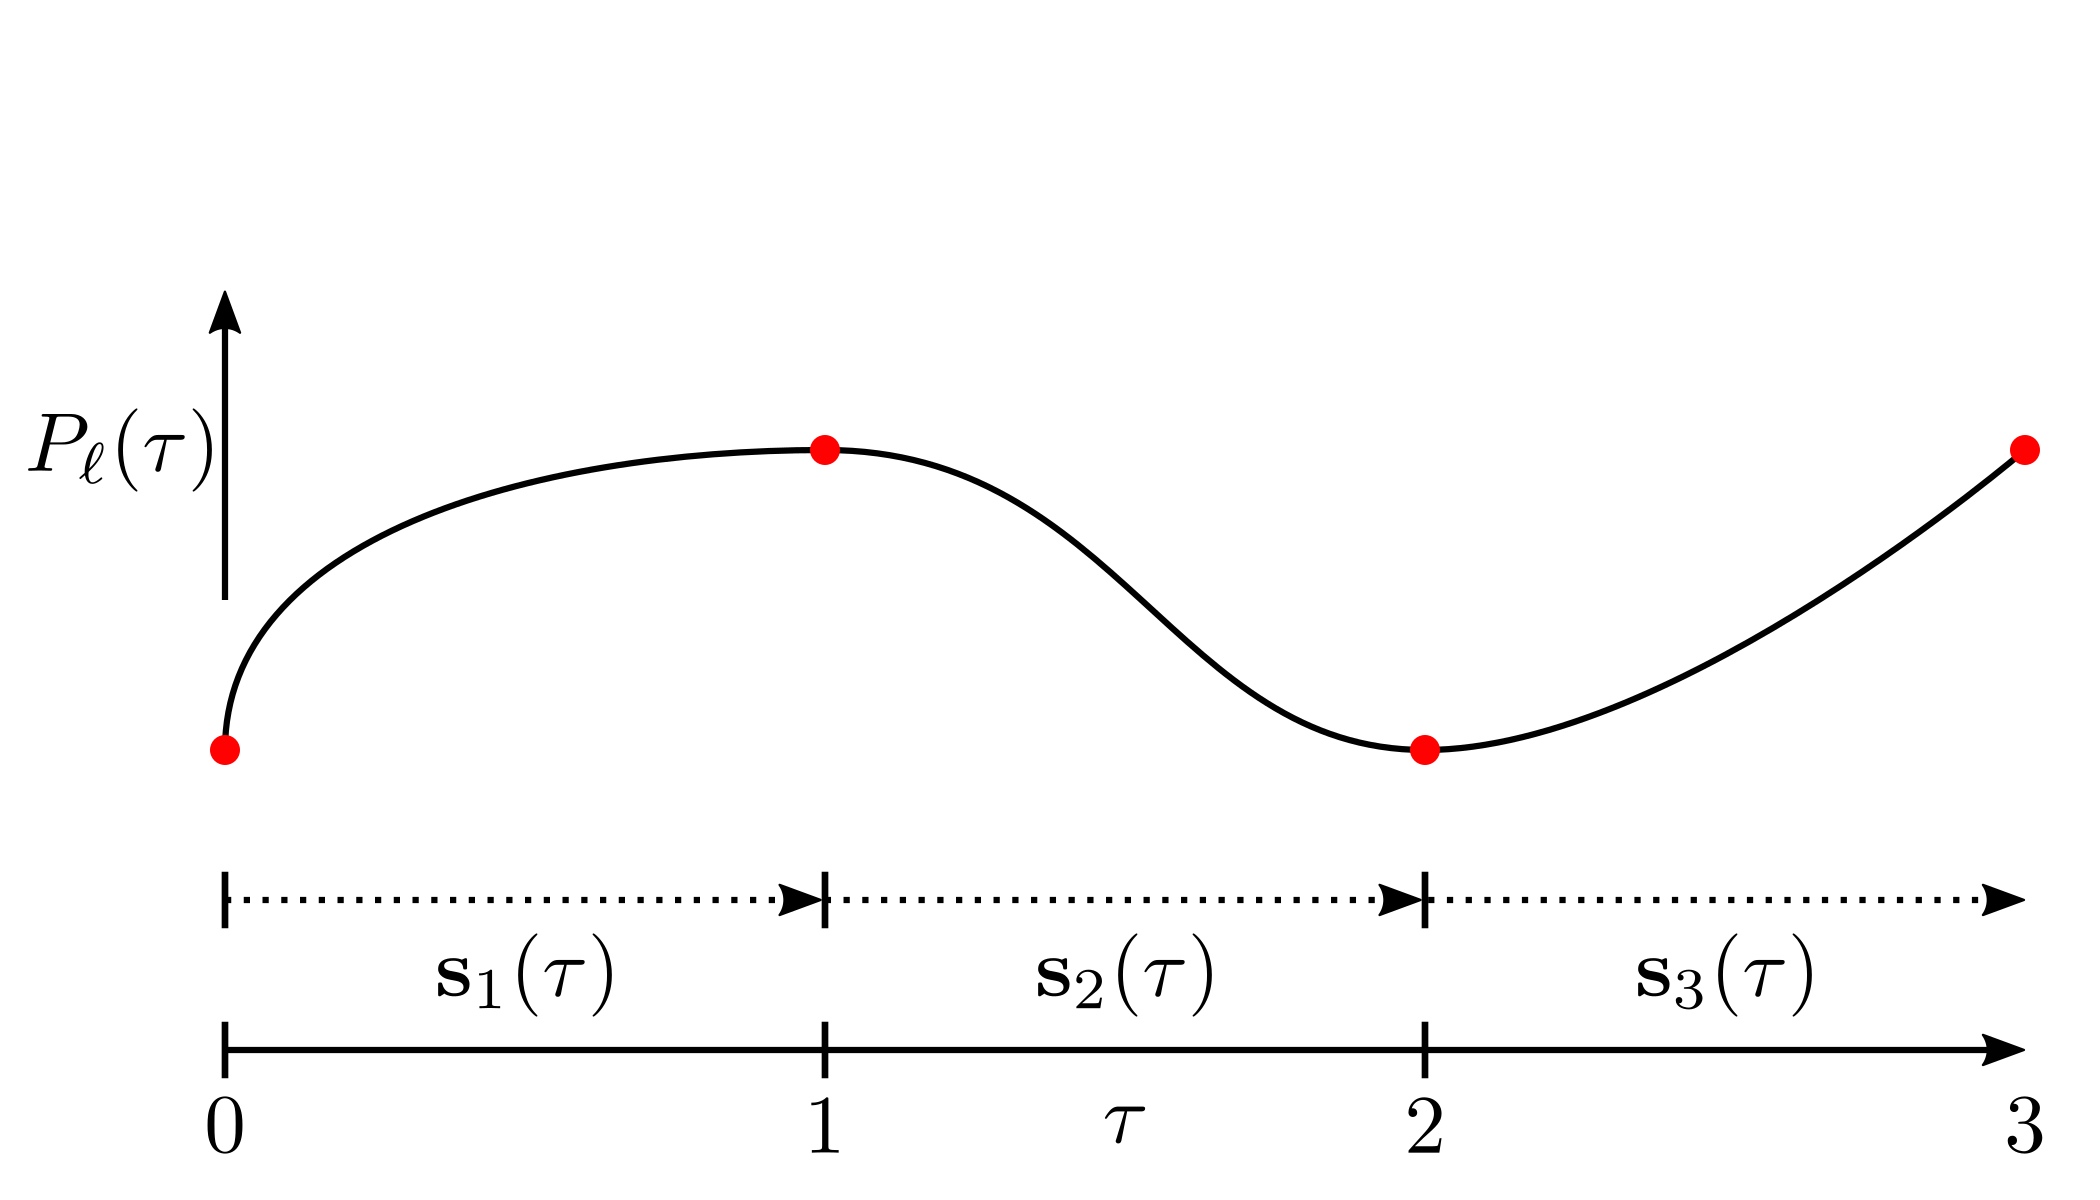
\includegraphics[width=\linewidth]{chap5_trajectory_planning/figures/trajectory_notation}
%	\caption{Notation used for a single spline.}
%	\label{fig:norm_accel_sol}
%\end{figure*}
%
%Let $P(\tau) = (P_1(\tau), P_2(\tau), \dots, P_r(\tau))$ be a set of $r$ splines, denoted $P_\ell(\tau)$, each of which is made up of $m$ segments, denoted $P_{\ell, i}(\tau)$,
%where $\tau \in [0, m]$.
%Each segment is parameterized by $s \in [0,1]$ and consists of the inner product of a vector of $n$ basis functions,
%\begin{equation}
%	\boldsymbol{\varphi}(s) = [\varphi_1(s), \varphi_2(s), \dots, \varphi_n(s)]^\top
%\end{equation}
%with $n$ coefficients $p_{\ell, i, j}$.
%\marginnote{
%	Choices for basis functions include the standard polynomials  
%	$\boldsymbol{\varphi}(s) = [1, s, s^2, \dots, s^{n-1}]$, or the Legendre polynomials.
%	Our implementation currently uses the standard polynomials.
%}
%We use a uniform spacing between segments, switching when $\tau\: \mathrm{mod}\: 1 = 0$.
%To handle switching between segments, we define the basis vector for the $i^\text{th}$ segment as
%\begin{equation}
%	\mathbf{s}_i(\tau) = 
%	\begin{cases} 
%		\boldsymbol{\varphi}(s) & \text{for } i - 1 \leq \tau < i, \text{ with } s = \tau\: \mathrm{mod}\: i \\
%		\mathbf{0}_n & \text{otherwise}
%	\end{cases}
%\end{equation}
%where $\mathbf{0}_n$ is an $n \times 1$ vector of zeros.
%Similarly, we define the $k^\text{th}$ derivative of 
%$\mathbf{s}_i(\tau)$ with respect to $\tau$ as
% where
%\begin{equation}
%\mathbf{s}^{(k)}_i(\tau) \triangleq \frac{d^k \mathbf{s}(\tau)}{d\tau^k} = 
%	\begin{cases} 
%		\boldsymbol{\varphi}^{(k)} (s) & \text{for } i - 1 \leq \tau < i, \text{ with } s = \tau\: \mathrm{mod}\: i \\
%		\mathbf{0}_n & \text{otherwise}
%	\end{cases}
%\end{equation}
%where 
%\begin{equation}
%	\boldsymbol{\varphi}^{(k)} = [\varphi^{(k)}_1(s), \varphi^{(k)}_2(s), \dots, \varphi^{(k)}_n(s)]^\top
%\end{equation}
%and 
%\begin{equation}
%	\varphi_j^{(k)} \triangleq \frac{d^k\varphi}{ds^k}.
%\end{equation}
%Stacking these basis vectors, we get the $nm\times 1$ $\tau$-dependent vector
%\begin{equation}
%	\mathbf{S}(\tau) = 
%	\begin{bmatrix} 
%		\mathbf{s}_1(\tau)^\top, &
%		\mathbf{s}_2(\tau)^\top, &
%		\dots, &
%		\mathbf{s}_m(\tau)^\top
%	\end{bmatrix}^\top
%\end{equation}
%and
%\begin{equation}
%	\mathbf{S}^{(k)}(\tau) = 
%	\begin{bmatrix} 
%		\mathbf{s}_1^{(k)}(\tau)^\top, &
%		\mathbf{s}_2^{(k)}(\tau)^\top, &
%		\dots, &
%		\mathbf{s}_m^{(k)}(\tau)^\top
%	\end{bmatrix}^\top.
%\end{equation}
%Define the $n\times 1$ vector of segment coefficients for the $i^{\text{th}}$ segment of the $\ell^\text{th}$ spline to be
%\begin{equation}
%	\mathbf{p}_{\ell, i} = 
%	\begin{bmatrix}
%		p_{\ell, i, 1},& p_{\ell, i, 2},& \dots,& p_{\ell, i, n}
%	\end{bmatrix}^\top,
%\end{equation}
%the $n m \times 1$ vector of all segment coefficients for the $\ell^\text{th}$ spline to be
%\begin{equation}
%	\mathbf{p}_{\ell} = 
%	\begin{bmatrix}
%	\mathbf{p}_{\ell, 1}^\top,& \mathbf{p}_{\ell, 2}^\top,& \dots,& \mathbf{p}_{\ell, n}^\top 
%\end{bmatrix}^\top,
%\end{equation}
%and the $r \times n m$ matrix of segment coefficients for all splines to be 
%\begin{equation}
%	\mathbf{P} = 
%	\begin{bmatrix} 
%		\mathbf{p}_{1} &
%		\mathbf{p}_{2} &
%		\dots &
%		\mathbf{p}_{r}
%	\end{bmatrix}.
%\end{equation}
%Then, we can write 
%\begin{equation}
%	P_{\ell, i}(\tau) = \mathbf{p}_{\ell, i}^\top \mathbf{s}_i(\tau),
%\end{equation}
%\begin{equation}
%	P_{\ell, i}^{(k)}(\tau) = \mathbf{p}_{\ell, i}^\top \mathbf{s}_i^{(k)}(\tau),
%\end{equation}
%\begin{equation}
%	P_\ell(\tau) = \mathbf{p}_\ell^\top \mathbf{S}(\tau),
%\end{equation}
%\begin{equation}
%	P_\ell^{(k)}(\tau) = \mathbf{p}_\ell^\top \mathbf{S}^{(k)}(\tau),
%\end{equation}
%\begin{equation}
%	P(\tau) = \mathbf{P}^\top \mathbf{S}(\tau),
%\end{equation}
%and
%\begin{equation}
%	P^{(k)}(\tau) = \mathbf{P}^\top \mathbf{S}^{(k)}(\tau).
%\end{equation}
%
%\section{Satisfying knot point constraints}
%\label{sec:knotpoint}
%Knot point constraints ensure that the trajectory passes through desired waypoints, and that it is continuous at the desired knot points. 
%Additionally, these constraints can be used to fix the derivatives of the trajectory at knot points.
%This leads to two different types of constraints:
%ensuring continuity of a derivative between two connecting segments, 
%and fixing the value of a derivative at the endpoint of the segment. 
%These can be written as inner products between $\mathbf{p}_\ell$ and $mn \times 1$ 
%vectors consisting of zeros and one or more $\boldsymbol{\varphi}^{(k)}(s)$, evaluated at $0$ or $1$. 
%
%First, we define the $mn \times 1$ vector with $\boldsymbol{\varphi}^{(k)} (s)$ in the $i^\text{th}$ position and zeros elsewhere as
%\begin{equation}
%	\Phi^{(k)}_{i} (s) = [\mathbf{0}_{n(i-1)}^\top, \boldsymbol{\varphi}^{(k)} (s)^\top, \mathbf{0}_{m(n-i)}^\top]^\top.
%\end{equation}
%
%\begin{theorem}
%	Derivative continuity and knot point value constraints for a trajectory member $P_\ell(\tau)$ can be written as an inner product between 
%	$\Phi^{(k)}_{i} (s)$ and $\mathbf{p}_\ell$.
%\end{theorem}
%
%\proof
%	%Let $i = \floor{(\tau + 1)}$. Then, the values of $P_\ell(\tau)^{(k)}$ at its knot points are 
%	The value of the starting knot points of segments in $P_\ell(\tau)$ are
%	\begin{align}
%		\mathbf{p}_\ell^\top \Phi^{(k)}_i (0) & \text{ for } i \in [1, n]
%	\end{align}
%	and the value of the ending knot points of segments in $P_\ell(\tau)$ are
%	\begin{align}
%		\mathbf{p}_\ell^\top \Phi^{(k)}_i (1) & \text{ for } i \in [1, n].
%	\end{align}
%
%	Thus, the $k^\text{th}$ derivative at the initial knot point of a segment $i$ can be set to a value $a$ by enforcing the constraint
%	\begin{align}
%		\mathbf{p}_\ell^\top \Phi^{(k)}_i (0) = a,
%	\end{align}
%	and the $k^\text{th}$ derivative at the final knot point of a segment $i$ can be set to a value $a$ by enforcing the constraint
%	\begin{align}
%		\mathbf{p}_\ell^\top \Phi^{(k)}_i (1) = a.
%	\end{align}
%
%	Continuity of the $k^\text{th}$ derivative between segments $i$ and $i+1$ can be ensured while allowing the value to vary by enforcing
%	\begin{align}
%		&\mathbf{p}_\ell^\top \Phi^{(k)}_i (1) = \mathbf{p}_\ell^\top \Phi^{(k)}_{i+1} (0)\\
%		\Longleftrightarrow &\mathbf{p}_\ell^\top \Phi^{(k)}_i (1) - \mathbf{p}_\ell^\top \Phi^{(k)}_{i+1} (0) = 0\\
%		\Longleftrightarrow &\mathbf{p}_\ell^\top (\Phi^{(k)}_i (1) - \Phi^{(k)}_{i+1} (0)) = 0
%	\end{align}
%\endproof
%
%We let
%\begin{equation}
%\mathbf{a}_\ell^{(k_a)} = [a_{\ell,1}^{(k_a)}, a_{\ell,2}^{(k_a)}, \dots, a_{\ell,m+1}^{(k_a)}],
%\end{equation}
%denote the desired knot point locations ($k_a = 0$), or derivatives ($k_a > 0$) for the $\ell^\text{th}$ spline, 
%where $\mathbf{a}_\ell^{(k_a)} \in \mathbb{R}^{c_{k_a}}$, with $c_{k_a} \leq m+1$.
%It is possible to leave intermediate knot points free in their location or derivative, making $c_{k_a} < m+1$.
%We use the convention that knot point 1 refers to the first knot point in the trajectory, 
%and knot point $m+1$ refers to the final knot point.
%The location or derivative constraints can be represented in matrix form with
%\begin{equation}
%	D^{(k_a)} \mathbf{p}_\ell = \mathbf{a}^{(k_a)}_\ell,
%\end{equation}
%defining the $m+1 \times mn$ matrix
%\begin{equation}
%	D^{(k_a)} \triangleq \begin{bmatrix}
%		(\Phi^{(k_a)}_1(0))^\top \\
%		(\Phi^{(k_a)}_2(0))^\top \\
%		\vdots\\
%		(\Phi^{(k_a)}_m(1))^\top 
%	\end{bmatrix}.
%\end{equation}
%With $k_{a,\text{max}}$ being the highest derivative at which the value or derivatives of a knot point
%is fixed, we let
%\begin{equation}
%	\bar{\mathbf{a}}_\ell = \begin{bmatrix}
%		\mathbf{a}^{(0)}_\ell, \\
%		\mathbf{a}^{(1)}_\ell, \\
%		\vdots \\
%		\mathbf{a}^{(k_{a,\text{max}})}_\ell, \\
%	\end{bmatrix}
%\end{equation}
%whose length we denote to be $c_a$.
%
%
%Similarly, the intermediate knot point continuity constraints for the $k_\ell^\text{th}$ derivative can be represented in matrix form as
%\begin{equation}
%	D_c^{(k_\ell)} \mathbf{p}_\ell = \mathbf{0}_{m-1}
%\end{equation}
%with the $m-1 \times mn$ matrix
%\begin{equation}
%	D_c^{(k_\ell)} \triangleq \begin{bmatrix}
%		(\Phi^{(k_\ell)}_1 (1) - \Phi^{(k_\ell)}_{2} (0))^\top \\
%		(\Phi^{(k_\ell)}_2 (1) - \Phi^{(k_\ell)}_{3} (0))^\top \\
%		\vdots \\
%		(\Phi^{(k_\ell)}_{m-1} (1) - \Phi^{(k_\ell)}_{m} (0))^\top 
%	\end{bmatrix}.
%\end{equation}
%If $k_{\ell,\text{max}}$ is the highest order of derivative for which we wish to enforce continuity at the knot points,
%there will be $(m-1) k_{\ell,\text{max}}$ continuity constraints. 
%We then define
%\begin{equation}
%	\mathbf{a}_\ell = \begin{bmatrix} \bar{\mathbf{a}}_\ell \\ \mathbf{0}_{(m-1)k_{\ell,\text{max}}} \end{bmatrix}
%\end{equation}
%to be a vector of length $c = c_a + (m-1)k_{\ell,\text{max}}$, and the $c \times r$ matrix
%\begin{equation}
%\mathbf{A} = \begin{bmatrix} \mathbf{a}_1 & \mathbf{a}_2 & \dots & \mathbf{a}_r \end{bmatrix}
%\end{equation}.  
%We can then formulate the knot point constraints for all of the splines in matrix form as
%\begin{equation}
%	\label{eq:knot_con}
%	\mathbf{D} \mathbf{P} = \mathbf{A}
%\end{equation}
%where
%\begin{equation}
%	\mathbf{D} = 
%	\begin{bmatrix}
%		D^{(0)}\\
%		\vdots \\
%		D^{(k_{a,\text{max}})}\\
%		D_c^{(0)} \\
%		\vdots\\
%		D_c^{(k_{\ell, \text{max}})}
%	\end{bmatrix} \in \mathbb{R}^{c \times mn}.
%\end{equation}
%
%By choosing $n$ such that $mn > c$, $\mathbf{D}$ will be wide, and Eq.~\ref{eq:knot_con} will be an under determined system with $mn - c$ remaining degrees of freedom.
%We assume that $\rank{(\mathbf{D})} = c$; if $\rank{(\mathbf{D})} < c$, there are linearly dependent constraints that can be removed from $\mathbf{D}$.
%
%As shown in \cite{MoonStirling00}, the singular value decomposition (SVD)
%can be used to find the solution to Eq.~\ref{eq:knot_con} of minimum norm.
%Generally, the SVD of an $n \times m$ matrix $\mathbf{X}$ with rank $r$ is 
%\begin{equation}
%	\mathbf{X} = U \Sigma V^\top = 
%	\begin{bmatrix} U_1 & U_2 \end{bmatrix} 
%	\begin{bmatrix} \Sigma_1 & \\ & \Sigma_2 \end{bmatrix} 
%	\begin{bmatrix} V_1^\top \\ V_2^\top \end{bmatrix},
%	\label{eq:D_svd}
%\end{equation}
%where $U \in \mathbb{R}^{n \times n}$, $V \in \mathbb{R}^{m \times m}$, and $\Sigma \in \mathbb{R}^{n \times m}$, with
%$U_1 \in \mathbb{R}^{n \times r}$, $U_2 \in \mathbb{R}^{n \times (n-r)}$,
%$\Sigma_1 \in \mathbb{R}^{r \times r}$, $\Sigma_2 \in \mathbb{R}^{(n-r) \times (m-r)}$,
%$V_1 \in \mathbb{R}^{m \times r}$, and $V_2 \in \mathbb{R}^{m \times (m-r)}$.
%Noting that since $\rank{(\mathbf{D})} = c$, 
%\begin{equation}
%	\mathbf{D} = U \Sigma V^\top = 
%	U 
%	\begin{bmatrix} \Sigma_1 & \Sigma_2 \end{bmatrix} 
%	\begin{bmatrix} V_1^\top \\ V_2^\top \end{bmatrix},
%	\label{eq:D_svd}
%\end{equation}
%where $U \in \mathbb{R}^{c \times c}$, $V \in \mathbb{R}^{mn \times mn}$, and $\Sigma \in \mathbb{R}^{c \times mn}$, with
%$\Sigma_1 \in \mathbb{R}^{c \times c}$, $\Sigma_2 \in \mathbb{R}^{c \times mn-c}$,
%$V_1 \in \mathbb{R}^{mn \times c}$, and $V_2 \in \mathbb{R}^{mn \times (mn-c)}$.
%Because it is not of full column rank, $\mathbf{D}$ has a nontrivial nullspace which is spanned by the columns of $V_2$.
%Solutions to Eq.~\ref{eq:knot_con} are then
%\begin{equation}
%	\label{eq:P_svd_sol}
%	\mathbf{P} = \bar{\mathbf{P}} + V_2 \mathbf{B} = V_1 \Sigma_1^{-1} U^\top \mathbf{A} + V_2 \mathbf{B}
%\end{equation}
%where $\bar{\mathbf{P}}$ is the minimum norm solution to Eq.~\ref{eq:knot_con}, and $\mathbf{B} \in \mathbb{R}^{(mn-c) \times r}$.
%
%Thus, a polynomial trajectory satisfying the constraints given by $\mathbf{D}$ and $\mathbf{A}$ is
%\begin{equation}
%	P(\tau) = \mathbf{P}^\top \mathbf{S}(\tau).
%\end{equation}

\section{Minimizing the $k^\mathrm{th}$ derivative}
Beyond satisfying knot point constraints, it is common \cite{RichterBryRoy16,MellingerKumar11} 
to minimize the integral of some derivative $k_r$ of $P(\tau)$ over the length of the trajectory,
\begin{equation}
	\label{eq:min_derivative}
	\begin{aligned}
	&\min_{\mathbf{P}} \int_{0}^m \|P^{(k_r)}(\tau)\|^2 d\tau \\
	&\text{subject to } \: \mathbf{D}\mathbf{P} = \mathbf{A}. 
	\end{aligned}
\end{equation}
The choice of $k_r$ is typically chosen to be one higher than the highest derivative needed to perform control. 
For a quadroter, snap ($k_r = 4$) is often minimized~\cite{MellingerKumar11}.


We now consider the solution to this optimization.
\begin{theorem}
	With 
	\begin{equation}
		\mathbf{W} \triangleq \int_0^m \mathbf{S}^{(k_r)}(\tau) (\mathbf{S}^{(k_r)} (\tau))^\top d\tau
	\end{equation}
	the optimization in Eq.~\ref{eq:min_derivative} has the analytic solution
	\begin{equation}
		\mathbf{P}^\star = \mathbf{H} \mathbf{A}
	\end{equation}
	where
	\begin{equation}
		 \mathbf{H}  = (\mathbf{I}_{mn \times mn} - V_2(V_2^\top \mathbf{W} V_2)^{-1} V_2^\top \mathbf{W})V_1 \Sigma^{-1} U^\top.
	\end{equation}
\end{theorem}
\proof
	As indicated by Eq.~\ref{eq:P_svd_sol}, there are infinitely many trajectories satisfying Eq.~\ref{eq:knot_con}.
	By modifying $\mathbf{B}$, the remaining degrees of freedom in Eq.~\ref{eq:knot_con} can be utilized to achieve a secondary objective. 
	To this end, we reformulate Eq.~\ref{eq:min_derivative} to be an unconstrained optimization over $\mathbf{B}$:
	\begin{equation}
		\label{eq:min_derivative_uncon}
		\begin{aligned}
		&\min_{\mathbf{B}} \int_{0}^m \|P^{(k_r)}(\tau)\|^2 d\tau. 
		\end{aligned}
	\end{equation}
	We then have
	\begin{align}
		&\min_{\mathbf{B}} \int_{0}^m \|P^{(k_r)}(\tau)\|^2 d\tau \\
		&= \min_{\mathbf{B}} \int_{0}^m (\mathbf{P}^\top \mathbf{S}^{(k_r)}(\tau))^\top \mathbf{P}^\top \mathbf{S}^{(k_r)}(\tau)  d\tau \\
		&= \min_{\mathbf{B}} \int_{0}^m (\mathbf{P}^\top \mathbf{S}^{(k_r)}(\tau))^\top \mathbf{P}^\top \mathbf{S}^{(k_r)}(\tau)  d\tau \\
		&= \min_{\mathbf{B}} \int_{0}^m  (\mathbf{S}^{(k_r)}(\tau)^\top \mathbf{P} \mathbf{P}^\top \mathbf{S}^{(k_r)}(\tau)  d\tau \\
		&= \min_{\mathbf{B}} \mathrm{tr} \left\{ \int_{0}^m  (\mathbf{S}^{(k_r)}(\tau)^\top \mathbf{P} \mathbf{P}^\top \mathbf{S}^{(k_r)}(\tau)  d\tau \right\} \\
		&= \min_{\mathbf{B}} \mathrm{tr} \left\{ \int_{0}^m \mathbf{P}^\top \mathbf{S}^{(k_r)}(\tau)  (\mathbf{S}^{(k_r)}(\tau)^\top \mathbf{P}  d\tau \right\} \\
		&= \min_{\mathbf{B}} \mathrm{tr} \left\{ \mathbf{P}^\top \mathbf{W} \mathbf{P}  \right\}
	\end{align}
	where
	\begin{equation}
		\mathbf{W} \triangleq \int_0^m \mathbf{S}^{(k_r)}(\tau) (\mathbf{S}^{(k_r)} (\tau))^\top d\tau. 
	\end{equation}
	Noting that $\mathbf{W}$ is independent of $\mathbf{B}$, it can be seen that this optimization takes a quadratic form.

	Substituting $\mathbf{P} = \bar{\mathbf{P}} + V_2 \mathbf{B}$, we have
	\begin{align}
		&\min_{\mathbf{B}} \mathrm{tr} \left\{ \mathbf{P}^\top \mathbf{W} \mathbf{P}  \right\} \\
		&= \min_{\mathbf{B}} \mathrm{tr} \left\{ (\bar{\mathbf{P}} + V_2\mathbf{B})^\top \mathbf{W} (\bar{\mathbf{P}} + V_2\mathbf{B})  \right\}\\
		&= \min_{\mathbf{B}} \mathrm{tr} \left\{ (\bar{\mathbf{P}} + V_2\mathbf{B})^\top \mathbf{W} (\bar{\mathbf{P}} + V_2\mathbf{B})  \right\}\\
		&= \min_{\mathbf{B}} \mathrm{tr} \left\{ (\bar{\mathbf{P}})^\top \mathbf{W}\bar{\mathbf{P}} + \mathbf{B}^\top V_2^\top \mathbf{W} V_2 \mathbf{B}
		+ 2 \mathbf{B}_\ell^\top V_2^\top \mathbf{W}\bar{\mathbf{P}} \right\}
	\end{align}
	which is quadratic in $\mathbf{B}$.
	Taking the gradient, $\frac{\partial}{\partial \mathbf{B}_\ell}$ we have
	\begin{align}
		&2 V_2^\top \mathbf{W} V_2 \mathbf{B} + 2 V_2^\top \mathbf{W}\bar{\mathbf{P}}.
	\end{align}
	Setting to zero, we find that
	\begin{align}
		\mathbf{B}^\star = - (V_2^\top \mathbf{W} V_2)^{-1} V_2^\top \mathbf{W} \bar{\mathbf{P}}.
	\end{align}
	Now,
	\begin{align}
		\mathbf{P}^\star &= \bar{\mathbf{P}} + V_2 \mathbf{B}^\star \\
		&= (\mathbf{I}_{mn \times mn} - V_2  (V_2^\top \mathbf{W} V_2)^{-1} V_2^\top \mathbf{W}) \bar{\mathbf{P}}\\
		&= (\mathbf{I}_{mn \times mn} - V_2  (V_2^\top \mathbf{W} V_2)^{-1} V_2^\top \mathbf{W}) V_1 \Sigma^{-1} U^\top A
	\end{align}

\endproof

We now investigate the structure of $\mathbf{W}$ in more detail.
Letting $\mathbf{s}_i^{(k_r)}(\tau) = \mathbf{s}_i$ we have
\begin{align}
	\mathbf{W} &\triangleq \int_0^m \mathbf{S}^{(k_r)}(\tau) (\mathbf{S}^{(k_r)} (\tau))^\top d\tau. \\
	&= \int_0^m 
	\begin{bmatrix}
		\mathbf{s}_1 \\		
		\mathbf{s}_2 \\		
		\vdots \\
		\mathbf{s}_m
	\end{bmatrix}
	\begin{bmatrix}
		\mathbf{s}_1 &
		\mathbf{s}_2 &
		\dots &
		\mathbf{s}_m 
	\end{bmatrix} d\tau \\
	&= \int_0^m 
	\begin{bmatrix}
		\mathbf{s}_1 \mathbf{s}_1^\top & \mathbf{s}_1 \mathbf{s}_2^\top & \dots & \mathbf{s}_1 \mathbf{s}_m^\top\\		
		\mathbf{s}_2 \mathbf{s}_1^\top & \mathbf{s}_2 \mathbf{s}_2^\top & \dots & \mathbf{s}_2 \mathbf{s}_m^\top\\		
		\vdots & \vdots & \ddots & \vdots \\
		\mathbf{s}_m \mathbf{s}_1^\top & \mathbf{s}_m \mathbf{s}_2^\top & \dots & \mathbf{s}_m \mathbf{s}_m^\top\\		
	\end{bmatrix} d\tau. 
	\label{eq:int_s_grammian_full}
\end{align}
Since $\mathbf{s}^{(k_r)}_i(\tau) = \mathbf{0}_n$ for $\tau \not\in [i, i+1]$, and 
$\mathbf{s}^{(k_r)}_i(\tau) = \boldsymbol{\varphi}^{(k_r)}(s)$ for $\tau \in [i, i+1]$ with $s = \tau\:\text{mod}\:i$,
the cross terms $\mathbf{s}_i \mathbf{s}_j^\top$ for $i \neq j$ in Eq.~\ref{eq:int_s_grammian_full} evaluate to zero.
This makes $\mathbf{W}$ block diagonal.
Additionally, each of the diagonal terms is identical, giving us $\mathbf{W} = \mathrm{diag}(W, W, \dots, W)$, where
${W} \in \mathbb{R}^{n \times n}$ is the integral of a diagonal term of Eq.~\ref{eq:int_s_grammian_full}:
\begin{align}
	&{W} \triangleq \int_0^m \mathbf{s}^{(k_r)}_i(\tau) (\mathbf{s}^{(k_r)}_i(\tau))^\top d\tau \\
	=& \int_0^1 \boldsymbol{\varphi}^{(k_r)}(s) (\boldsymbol{\varphi}^{(k_r)}(s))^\top ds \\
	=& \int_0^1 
	\begin{bmatrix}
		(\varphi_1^{(k_r)}(s))^2 & \varphi_1^{(k_r)}(s) \varphi_2^{(k_r)}(s) & \dots & \varphi_1^{(k_r)}(s) \varphi_n^{(k_r)}(s)\\		
		\varphi_2^{(k_r)}(s) \varphi_1^{(k_r)}(s) & (\varphi_2^{(k_r)}(s))^2 & \dots & \varphi_2^{(k_r)}(s) \varphi_n^{(k_r)}(s)\\		
		\vdots & \vdots & \ddots & \vdots \\
		\varphi_n^{(k_r)}(s) \varphi_1^{(k_r)}(s) & \varphi_n^{(k_r)}(s) \varphi_2^{(k_r)}(s) & \dots & (\varphi_n^{(k_r)}(s))^2\\		
	\end{bmatrix} ds. 
\end{align}
It can be seen that $W$ is symmetric, and positive semi-definite.
If the basis members $\varphi_j$ are orthogonal, then ${W}$ is diagonal. 
If $k_r > 0$ (which, in general, will be true), then $\varphi_j^{(k_r)} = 0$ for $j < k_r$, making ${W}$ singular.
\jbwcomment{I have found that $V_2^\top \mathbf{W} V_2$ is full rank, so I think there is some more investigation we can do here.}

%\jbwcomment{ This is a really interesting result (assuming my math is correct). What we really care about is finding $\mathbf{r}_\ell$, since that is what will actually be applied to the trajectory. In general, $\mathbf{W}$ will be singular. Additionally, $V_2^T\mathbf{W}$ will be $(mn - c) \times mn$ (tall), so solving here for $\mathbf{r}_\ell$ will be approximate - or will we just get $\mathbf{r} = 0$?. In that case, $\mathbf{W}$ is irrelevant, and we only need to find $\mathbf{b}_\ell$ such that $\|V_2 \mathbf{b}_\ell + \mathbf{p}^\star_\ell\|$ is minimized, ie $\mathbf{b}_\ell = -V_2^\dagger \mathbf{p}$. That's a pretty cool result if that is the case, as it would also imply that it is true for minimizing any derivative - including the zeroth, so the minimum snap trajectory would also be minimum accel, velocity, and length.}



%--------------------------------------------------------------------------------
%--------------------------------------------------------------------------------
%--------------------------------------------------------------------------------

\section{Ensuring dynamic feasibility using time scaling}
The dynamics of a differentially flat system can be satisfied by planning in the flat output space. 
However, these dynamic models typically neglect system limitations such as actuator saturation. 
It is possible to include system limits in the trajectory optimization. 
These limits typically yield non-convex constraints, requiring a nonlinear optimizer to solve.
Instead of directly constraining the system, we use time scaling to ensure the constraints are satisfied.

Let 
\begin{equation}
\tau = \alpha t, 
\end{equation}
where $t$ is dimensional time. 
We then define the trajectory $P(t) = P(\tau(t))$, and the system dynamic constraints to be a nonlinear function of the trajectory and its derivatives:
\begin{equation}
	C(P(t), P^{(1)}(t), \dots, P^{(k)}(t)).
\end{equation}

\begin{theorem}
	The derivatives of $P(t)$ with respect to $t$ can be written as
	\begin{equation}
		\frac{d^{k}} {dt^k}  = \alpha^k \frac{d^k P}{d\tau^k}
	\end{equation}
\end{theorem}
\proof
Should probably be by induction\dots

With $P(t) = P(\alpha t)$, and noting that $\frac{d\tau}{dt} = \alpha$, by the chain rule we have
\begin{align}
\frac{dP}{dt} &= \frac{dP}{d\tau}\frac{d\tau}{dt} = \alpha \frac{dP}{d\tau} \\
\frac{d^2P}{dt^2} &= \frac{d}{dt} \left( \alpha \frac{dP}{d\tau} \right) = \alpha \frac{d^2P}{d\tau^2}\frac{d\tau}{dt} = \alpha^2 \frac{d^2P}{d\tau^2}  \\
\frac{d^3P}{dt^3} &= \frac{d}{dt} \left( \alpha^2 \frac{d^2P}{d\tau^2} \right) = \alpha^2 \frac{d^3P}{d\tau^3}\frac{d\tau}{dt} = \alpha^3 \frac{d^3P}{d\tau^3} \\
&\vdots
\end{align}
\endproof

%%% end Jacob Willis stuff




\rwbcomment{Replace this section with Jacob Willis' stuff.}

If a system is differentially flat with flat output $z$, then the open-loop path planning problem presumably becomes much easier.  If there are no constraints on the state and input variables, then planning becomes trivial.  If there are constraints, then the planning problem can be reduced to a constrained optimization problem.

%+++++++++++++++++++++++++++++++++++++++++++++++++
\subsection{Path planning without constraints}
Suppose that the objective is to plan a path from a start position $p_s$ and a start velocity $p_s^{'}$, to an end position $p_e$ and an end velocity $p_e^{'}$.  Instead of parameterizing the path by time $t$, we will use the path parameter $\sigma$.  This will allow us to later specify the velocity by creating dynamics for $\sigma(t)$.  Let  $p:[0,T]\to\re^3$ denote the path.  The path will be given by the finite series expansion
\begin{align*}
p(\sigma) &= \begin{pmatrix} \sum_{j=1}^N c_{1j} \phi_j(\sigma) \\  \sum_{j=1}^N c_{2j} \phi_j(\sigma) \\  \sum_{j=1}^N c_{3j} \phi_j(\sigma) \end{pmatrix} \\
&= C\phi(t),
\end{align*}
where 
\[
C = \begin{pmatrix} c_{11} & c_{12} & \dots & c_{1N} \\ c_{21} & c_{22} & \dots & c_{2N} \\c_{31} & c_{32} & \dots & c_{3N} \end{pmatrix},
\]
and
\[
\phi(\sigma) = \begin{pmatrix} \phi_1(\sigma) & \phi_2(\sigma) & \dots & \phi_N(\sigma) \end{pmatrix}^{\top},
\]
and where $\{\phi_j(\sigma)\}$ are the basis functions.  For example, for a polynomial basis we have $\phi_j(\sigma)=\sigma^j/j!$. We also define the derivative of the basis function as
\[
\phi_j^{'}(\sigma)\defeq\frac{d\phi_j}{d\sigma}(\sigma),
\]
and 
\[
\phi^{'}(\sigma) = \begin{pmatrix} \phi_1^{'}(\sigma) & \phi_2^{'}(\sigma) & \dots & \phi_N^{'}(\sigma) \end{pmatrix}^{\top}.
\]

For the path the start at $p_s$ we must have
\[
p_s = p(0)= C\phi(0).
\]
For the start velocity to be $p_s^{'}$ we must have
\[
p_s^{'} = p^{'}(0) = C\phi^{'}(0).
\]
For the path to end at $p_e$ we need
\[
p_e = p(T)= C\phi(T),
\]
and for the end velocity to be $p_e^{'}$ we require that
\[
p_e^{'} = p^{'}(T) = C\phi^{'}(T).
\]
Since $\sigma$ is a path parameterization, without loss of generality we will let $\sigma$ at the endpoint equal to $T=1$.

Defining 
\begin{align*}
P &\defeq \begin{pmatrix} p_s & p_s^{'} & p_e & p_e^{'} \end{pmatrix} \\
\Phi &\defeq \begin{pmatrix} \phi(0) & \phi^{'}(0) & \phi(1) & \phi^{'}(1) \end{pmatrix}
\end{align*}
we have that the coefficients $C$ must satisfy
\begin{equation}\label{eq:flat-coefficient-equation}
C\Phi = P.  
\end{equation}

Let the singular value decomposition for $\Phi$ be given by $\Phi = \begin{bmatrix}U_1 & U_2\end{bmatrix}\begin{bmatrix}\Sigma \\ \mathbf{0} \end{bmatrix}V^\top = U_1\Sigma V^\top$, where 
$U_1\in\mathbb{R}^{N\times 4}$, $U_2\in\mathbb{R}^{N\times (N-4)}$, $\Sigma\in\mathbb{R}^{4\times 4}$, and $V\in\mathbb{R}^{4\times 4}$, and where $U_1^\top U_1 = I$, $U_2^\top U_2=I$, $U_1^\top U_2 = 0$, and $U_2^\top U_1=0$.  Letting
\[
C = PV\Sigma^{-1}U_1^\top + BU_2^\top,
\]
where $B\in\mathbb{R}^{3\times (N-4)}$ can be arbitrarily selected, then 
\begin{align*}
C\Phi &= (PV\Sigma^{-1}U_1^\top + BU_2^\top)U_1\Sigma V^\top \\
      &= PV\Sigma^{-1}\Sigma V^\top = P V V^\top \\
      &= P.
\end{align*}

The first term $PV\Sigma^{-1}U_1^\top$ is the minimum norm solution to the path planning problem.  The second term $BU_2^\top$ represents a parameterization of the corresponding null space.  Given additional constraints, the matrix $B$ can be selected to satisfy those constraints.


%+++++++++++++++++++++++++++++++++++++++++++++++++
\subsection{Time Parameterization}
The path can be time parameterized by letting $\sigma$ be a function of time, where we require that $\frac{d\sigma}{dt}>0$ to ensure a forward looking parameterization of the path.  If we desire a fixed speed $v^d$ along the path, then 
\begin{align*}
v^d &= \norm{\frac{d}{dt}p(\sigma(t))} \\
&= \norm{\frac{\partial p}{\partial\sigma}\frac{d\sigma}{dt}} \\
&= \norm{C\phi'(\sigma(t))}\frac{d\sigma}{dt}.
\end{align*}
Therefore, $\sigma$ should satisfy the differential equation
\[
\frac{d\sigma}{dt} = \frac{v^d}{\norm{C\phi'(\sigma(t))}}.
\]

The path length is dependent only on the parameter $\sigma$ and is given by
\begin{align*}
L &= \int_0^1 \norm{p'(\sigma)}d\sigma \\
  &= \int_0^1 \norm{C\phi'(\sigma)}d\sigma.
\end{align*}
Sampling $\sigma$ at a finite number of values $0\leq\sigma_1\leq\sigma_2\leq\dots\leq\sigma_N\leq 1$, the path length is approximated as
\[
L \approx \sum_{i=2}^N \norm{C\phi'(\sigma_i)}\abs{\sigma_i-\sigma_{i-1}}.
\]

    


%+++++++++++++++++++++++++++++++++++++++++++++++++
\subsection{Path planning with constraints}


If $N>4$, then $\Phi^\top$ has a non-trivial null space that can be exploited to satisfy additional constraints.  As an example, we may want to minimize the curvature of the path.  

The curvature of $p(\sigma)$ is defined by the formula
\[
\kappa(\sigma) = \frac{p^{'}(\sigma)\times p^{''}(\sigma)}{\norm{p^{'}(\sigma)}^3}.
\]
Since the path $p(\sigma)$ is also a function of the null space parametrization $B$, we write $p(\sigma, B)$, and so
\[
\kappa(\sigma, B) = \frac{p^{'}(\sigma, B)\times p^{''}(\sigma, B)}{\norm{p^{'}(\sigma, B)}^3}.
\]
To solve the path planning problem subject to a minimum curvature constraint, we need to solve the following optimization problem:
\[
B^\ast = \arg\min_{B\in\mathbb{R}^{3\times(N-4)}} \left\{ \max_{\sigma\in[0,1]}\kappa(\sigma, B)\right\}.
\]
To make the problem tractable, we can sample $\sigma$ at a finite number of values $0\leq\sigma_1\leq\sigma_2\leq\dots\leq\sigma_N\leq 1$, and solve
\[
B^\ast = \arg\min_{B\in\mathbb{R}^{3\times(N-4)}} \left\{ \max_{i=1,\dots,N}\kappa(\sigma_i, B)\right\}.
\]

\subsection{Minimum Snap Trajectory Generation and Control for Quadrotors, ICRA, 2011}
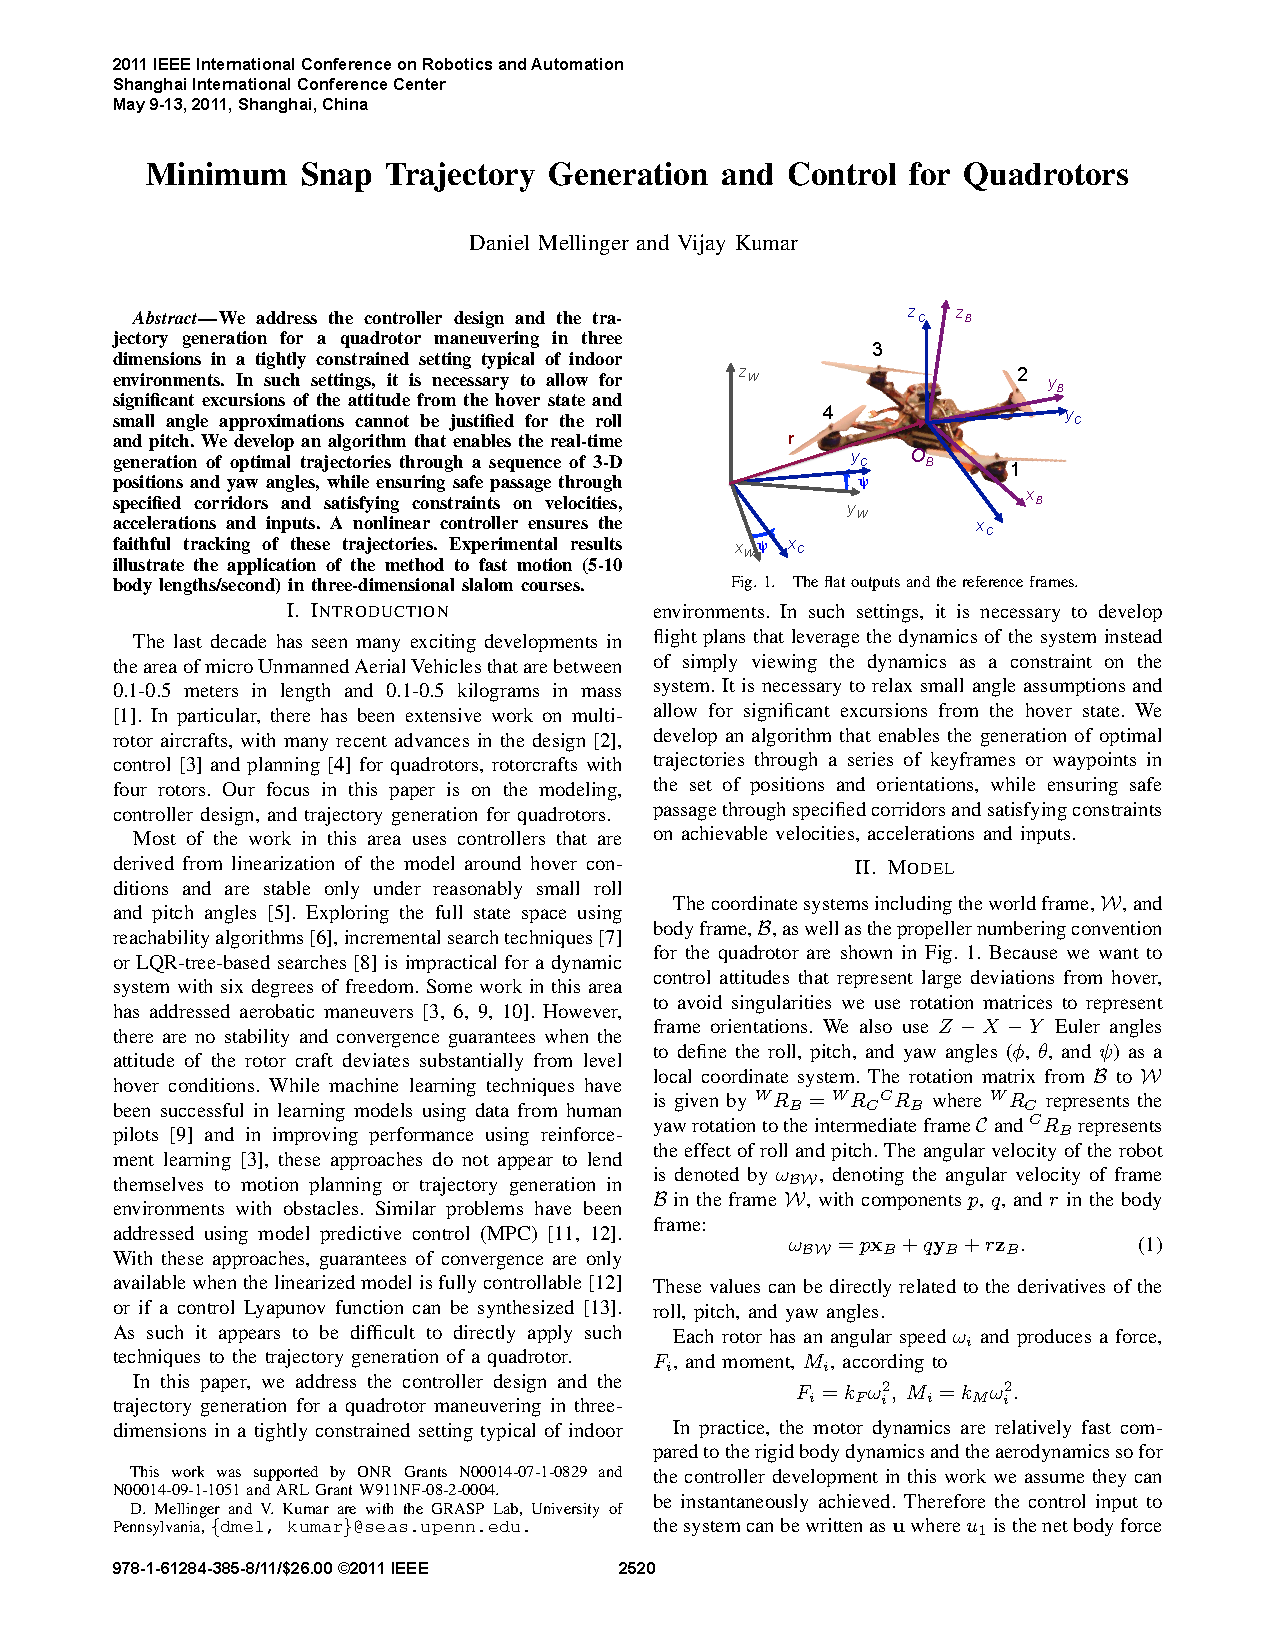
\includepdf[pages=-,scale=.8,pagecommand={}]{chap5_trajectory_planning/papers/MellingerKumar11.pdf}


%----------------------------------
\section{Path Planning using a Digital Elevation Map}

Add a discussion similar to this paper.
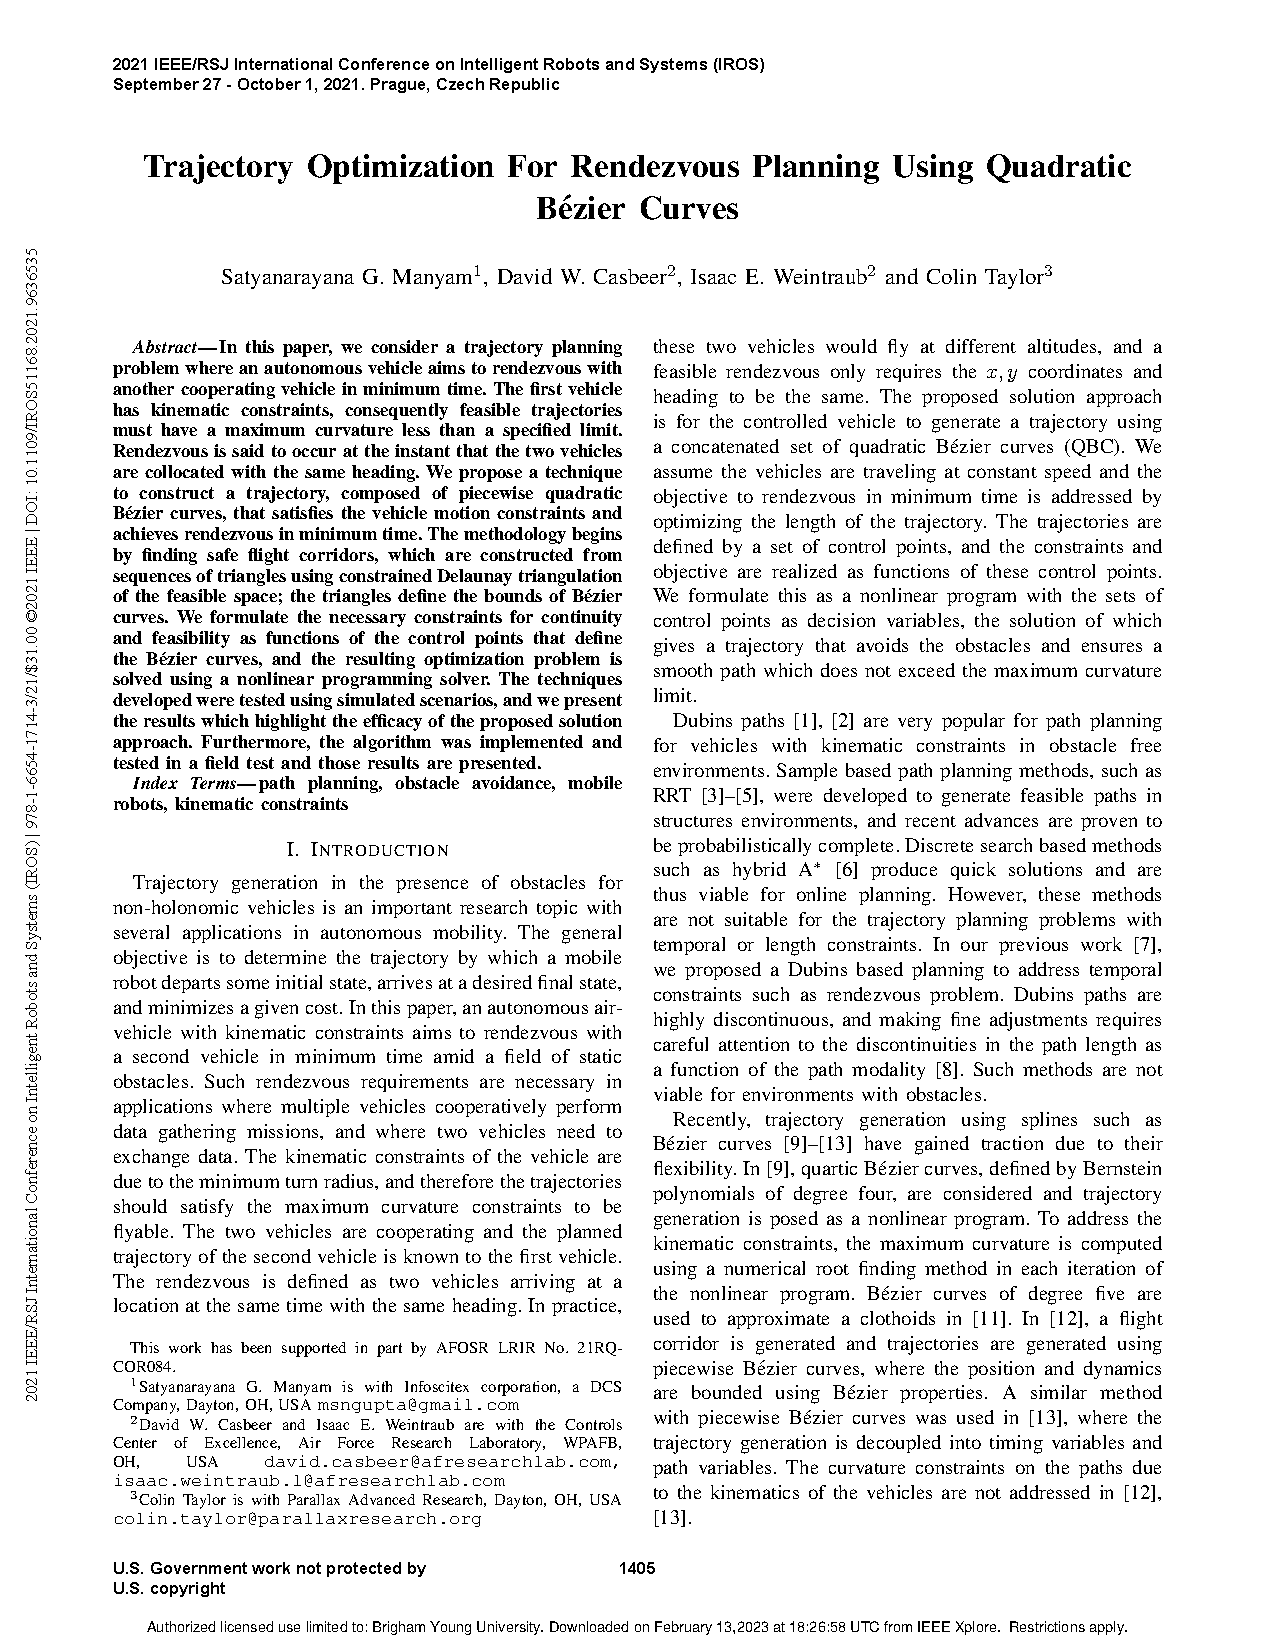
\includepdf[pages=-,scale=.8,pagecommand={}]{chap5_trajectory_planning/papers/ManyamCasbeerWeintraub21.pdf}


%%----------------------------------
%\section{Voxel map}
%
%\rwbcomment{Add Thane's stuff here.}
%
%\subsection{OctoMaps}
%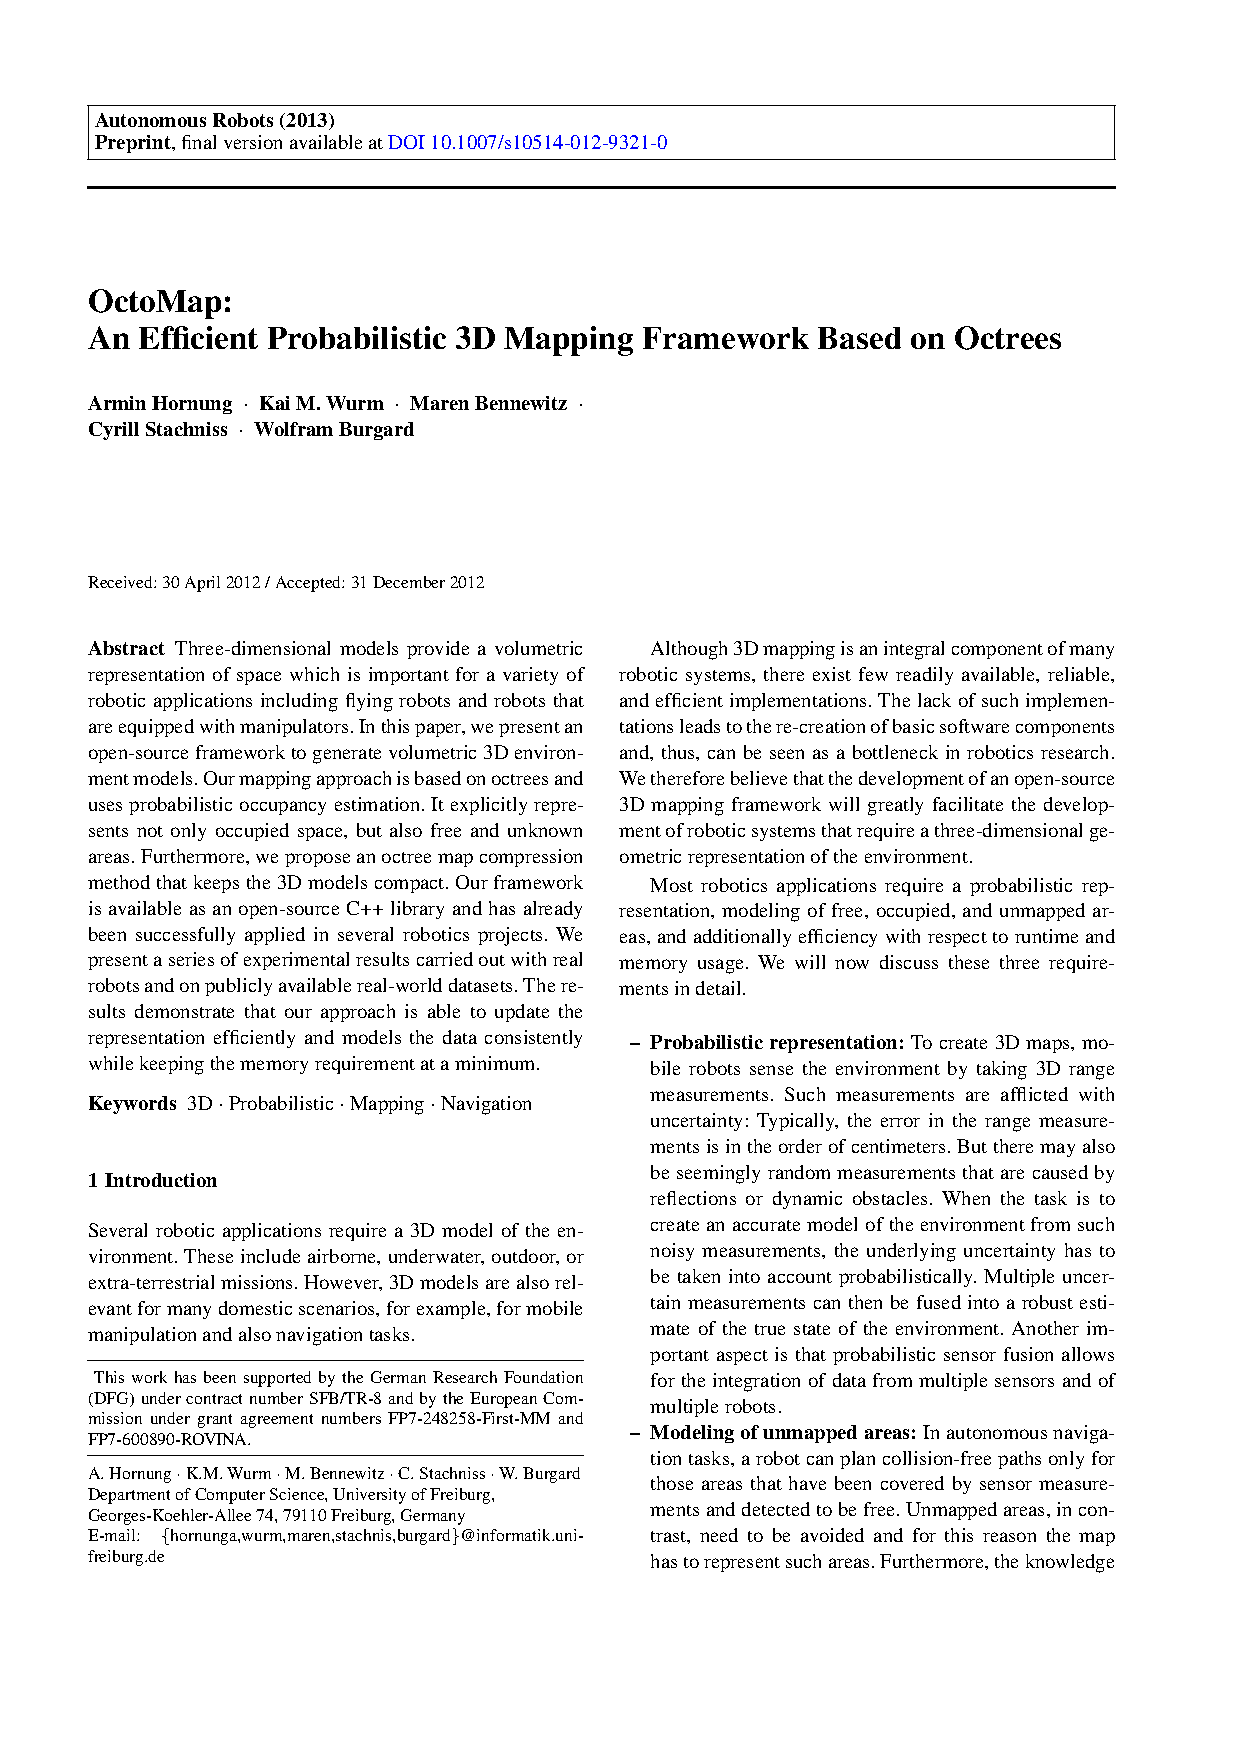
\includepdf[pages=-,scale=.8,pagecommand={}]{chap5_trajectory_planning/papers/Octomap.pdf}


%%----------------------------------
%\section{Waypoint planning in a voxel map}
%
%\subsection{Graph searching methods}
%%
%\begin{marginfigure}
%  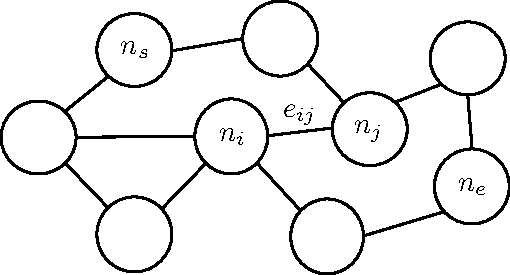
\includegraphics[width=\linewidth]{chap5_trajectory_planning/figures/plan-graph}
%  \caption{General graph structure for path planning.}
%  \label{fig:plan-graph}  
%\end{marginfigure}
%%
%We can model our world efficiently using discrete graphs where the nodes of the graph represent locations and the edges represent paths between locations. Typically we associate a cost with traveling along an edge from one node to the next. Figure~\ref{fig:plan-graph} shows a simple graph with a start node $n_s$, an end node $n_e$, and intermediate nodes $n_i$ and $n_j$. The cost for traveling along the edge from node $n_i$ to node $n_j$ is given by $e_{ij}$. Although not labeled, each edge has an associated cost. Edges can be unidirectional or bidirectional with with a uniform or different edge cost for each traversal direction. Edge costs can be used to represent proximity to obstacles, the physical distance between the two nodes, or other features of the environment. 
%
%The voxel maps described in the prior section can be represented as a graph structure where the center of the voxel is the node and cost for moving between adjacent voxels is the associated edge cost. To plan paths from a starting location in the voxel map to the specified goal location, we will utilize graph searching methods including widely used approaches such as Djikstra's algorithm and A* search.
%
%\vspace{1.0in}
%
%\rwbcomment{Add something like the following:}
%
%\href{https://www.redblobgames.com/pathfinding/a-star/introduction.html}{Introduction to A*}
%\href{https://brilliant.org/wiki/dijkstras-short-path-finder/}{Dijkstra's Algorithm}




